% ============================================================
%  JAL submission — enriched with deep EDA + 5 new figures
% ============================================================
\documentclass[review]{elsarticle}

\usepackage[utf8]{inputenc}
\usepackage[T1]{fontenc}
\usepackage{CJKutf8}
\usepackage{mathptmx}
\usepackage[scaled=.90]{helvet}
\usepackage{courier}
\usepackage{graphicx}
\usepackage{booktabs}
\usepackage{multirow}
\usepackage{enumitem}
\usepackage{hyperref}
\usepackage{setspace}
\onehalfspacing

\journal{The Journal of Academic Librarianship}

\begin{document}

\begin{frontmatter}

\title{From Individual Chronologies to Institutional Memory:\\\\
       Computational Curation of Scientist Oral History\\\\
       through Knowledge Graphs and Five Quality Metrics}

\begin{abstract}
Oral history constitutes a vital but methodologically under-examined component of library special collections. Unlike institutional records, oral testimonies carry intrinsic uncertainty, memory bias, and narrative isolation that challenge traditional cataloging and quality assessment. This study applies large language model (LLM)-based semantic extraction and multi-relational knowledge graph analysis to 26 chronological biographies (nianbiao) of Chinese senior scientists (born 1898--1935), comprising 2,582 discrete life events, to address three questions: (1) Can oral history collection quality be computationally quantified? (2) What gaps exist between special collections and public knowledge graphs? (3) Does enrichment with public data improve quality metrics? We develop a three-tier hybrid extraction architecture combining deterministic regex with LLM deep extraction (97.5\% education precision, 88.7\% award precision) and propose five computable quality indicators: Uncertainty Density (UD, range 1.12--5.96 markers/1K chars), Memory Bias Index (MBI, $\chi^2 = 842.2$, $p < 10^{-172}$), Cross-Reference Connectivity (CRC = 0.0\%), Narrative Arc Type (NAT, 57.7\% TRIUMPH), and Wikidata Enrichment Ratio (WER = 36.8$\times$). Comparison with Wikidata—measured against a full 142~GB Wikidata JSON dump—reveals that mentorship, collaboration, and biographical events—three relationship types critical to scientific biography—are entirely absent from the public knowledge graph for this cohort, while LLM extraction recovers 74 mentors, 268 collaborators, and 523 key life events. Projecting post-enrichment alignment, publishing these data would contribute approximately 1,717 net-new linked data statements at \$0.0007 per fact. We argue that the MI1--MI5 indicator system forms a closed-loop curatorial framework: libraries assess oral history quality (RQ1), identify Wikidata complementarity gaps (RQ2), publish enrichment data, then re-evaluate whether indicators improve or warrant further follow-up (RQ3). This transforms academic libraries from passive collection custodians into active linked data publishers with a quantifiable, iterative quality assurance process for oral history special collections.
\end{abstract}

\begin{keyword}
academic libraries \enspace$\bullet$\enspace special collections \enspace$\bullet$\enspace scientist archives \enspace$\bullet$\enspace knowledge graph \enspace$\bullet$\enspace chronologies \enspace$\bullet$\enspace nianbiao \enspace$\bullet$\enspace digital curation \enspace$\bullet$\enspace China
\end{keyword}

\end{frontmatter}

% ============================================================
\section{Introduction}
% ============================================================

Academic libraries occupy a unique position at the intersection of heritage preservation and knowledge discovery. Through special collections and archives, libraries collect, curate, and provide access to the personal papers, correspondence, and biographical materials of scientists \cite{oneill2019special,dooley2010taking}. These collections serve as institutional memory, connecting past scientific achievements to contemporary research communities and enabling historical inquiry into the development of scientific disciplines.

Yet the organization of scientist archives has been criticized for privileging individual biography over network analysis \cite{kwasnik2019knowledge}. Archival finding aids typically describe collections as self-contained units, obscuring the mentorship, collaboration, and shared institutional affiliations that give scientific archives their full meaning \cite{trace2012evolution,trace2020information}. Biographical texts such as chronological biographies (nianbiao in Chinese tradition) are rich in latent relational data, but these connections remain embedded in unstructured text, inaccessible to computational discovery \cite{griffin2014text}.

This study addresses three research questions concerning the quality assessment of oral history-based special collections and their relationship with public knowledge graphs:

\begin{enumerate}[label=RQ\arabic*:,leftmargin=*]
    \item Can the content quality of oral history special collections be computationally quantified and assessed?
    \item What gaps exist between oral history special collections and public knowledge graphs such as Wikidata, and how can these collections complement public data?
    \item Does enrichment with public data improve collection quality metrics, and under what conditions does it warrant further curatorial follow-up?
\end{enumerate}

% ============================================================
\section{Literature Review}
% ============================================================

\subsection{Scientist Archives and Library Special Collections}

The collection of scientist papers in academic libraries has a well-established tradition. Major collections---the Archives of American Scientists at the American Institute of Physics, the Einstein Archives at the Hebrew University of Jerusalem, and the Newton Papers at Cambridge University Library---demonstrate the scholarly value of curated scientist archives \cite{hunter2017archives}. In China, the Chinese Academy of Sciences Archives and university libraries at Tsinghua, Peking, and Jiaotong Universities maintain significant scientist collections \cite{zhang2018scientific}.

The ``biographical turn'' in digital humanities has opened new possibilities for computational analysis of life narratives \cite{sherratt2020biographical}. Topic modeling, named entity recognition, and social network analysis have been applied to corpora from the Dictionary of National Biography to the China Biographical Database (CBDB) \cite{bol2015china}. Gottschalk and Demidova \cite{gottschalk2019eventkg} developed EventKG, an event-centric knowledge graph that generates biographical timelines, providing a computational framework that aligns naturally with the event-based structure of Chinese nianbiao. Liu and Wang \cite{liu2017matrix} demonstrated graph-based relationship inference on CBDB data, showing how computational methods can extract kinship and social ties from historical Chinese biographical records.

Recent work has explored the intersection of large language models and knowledge graphs. Pan et al.\ \cite{pan2023unifying} surveyed approaches to unifying LLMs and KGs, identifying entity extraction and relationship inference as especially promising applications. De Paiva and Rademaker \cite{depaiva2024brazilian} demonstrated a domain-specific history knowledge graph construction pipeline, showing that semi-automated extraction can transform unstructured historical texts into queryable linked data—a model directly relevant to scientist nianbiao collections. Lu et al.\ \cite{lu2025karma} proposed KARMA, a multi-agent LLM framework for automated knowledge graph enrichment that addresses the scalability challenges inherent in manual curation. Carriero et al.\ \cite{carriero2024human} conducted a human evaluation of procedural KG extraction with LLMs, finding that structured prompting significantly improves extraction quality—a finding directly informing our three-tier extraction design. Blanke and Riechert \cite{blanke2020rdf} demonstrated the feasibility of constructing RDF knowledge graphs for historical scholars, providing a prosopographical methodology that our work extends to modern scientists.

\subsection{The Nianbiao Tradition and Linked Data}

The Chinese nianbiao---chronological biography---originates in Song dynasty historiography and presents life events in strict temporal order with precise dates and institutional contexts \cite{twitchett1962chinese,wilkinson2018chinese}. This structured format maps intuitively to the event-centric data models of modern knowledge graphs. The nianbiao's origin as retrospectively compiled oral testimony connects it to the broader oral history tradition, whose methodological foundations were established by Thompson \cite{thompson2000voice} and whose narrative theory was developed by Portelli \cite{portelli1991death}. Initiatives like SNAC (Social Networks and Archival Context) and VIAF have demonstrated the feasibility of person-centric linked data \cite{larson2015connecting}, while the CIDOC-CRM ontology provides a conceptual framework for modeling biographical events and their institutional contexts \cite{doerr2003cidoc}.

\subsection{Narrative Studies in Oral History and Computational Curation}

The study of narrative structure in oral history has deep roots in both the humanistic and computational traditions. Portelli \cite{portelli1991death} established that oral testimonies are not merely factual records but constructed narratives shaped by memory, identity, and the interview context---a theoretical foundation that directly informs our treatment of nianbiao as curated retrospective accounts rather than objective chronicles. Thompson \cite{thompson2000voice} further argued that the narrative form of oral history is itself a source of evidence, encoding social meaning in its selection, sequencing, and emphasis of events.

In computational narrative studies, Reagan et al.\ \cite{reagan2016emotional} demonstrated that the emotional trajectories of stories follow six basic shapes (rags-to-riches, tragedy, man-in-a-hole, Icarus, Cinderella, Oedipus) through sentiment analysis of large text corpora, providing empirical evidence that narrative arcs are quantifiable and reproducible patterns rather than subjective interpretations. Jockers \cite{jockers2015syuzhet} developed computational tools for extracting sentiment trajectories from literary texts, showing that plot structures can be algorithmically detected and compared across works. These advances in computational narratology underpin our narrative arc classification (TRIUMPH, RESILIENCE, STEADY, ASCETIC) in Section~\ref{sec:oral}: the LLM-based classification is not an ad-hoc labeling but an operationalization of established narrative archetypes adapted to the specific genre constraints of Chinese scientific nianbiao.

Within library and information science, the ``narrative turn'' has gained traction as scholars recognize that traditional metadata schemas (Dublin Core, MARC) are ill-suited to capturing the temporal, affective, and structural dimensions of life narratives \cite{sherratt2020biographical}. Trainin et al.\ \cite{trainin2026testimony} recently proposed a scalable computational framework for comparing oral history archives, demonstrating that structural patterns across testimonies---including narrative arc distributions---constitute a new dimension of archival metadata. Our work extends this line of inquiry by integrating narrative arc classification into a broader, multi-indicator quality assessment system (MI1--MI5) that links the narrative characteristics of oral history collections to concrete curatorial actions: collection browsing, gap analysis, researcher filtering, and Wikidata enrichment prioritization.

% ============================================================
\section{Methodology}
% ============================================================

\subsection{Corpus}

The corpus consists of 26 nianbiao files of Chinese senior scientists. Table~\ref{tab:corpus} summarizes corpus characteristics. Scientists span birth years 1898--1935 (37-year range) and cover physics, biology, geology, medicine, engineering, and agricultural science.

\begin{table}[ht]
\centering
\caption{Corpus characteristics and extraction summary.}
\label{tab:corpus}
\begin{tabular}{lrlr}
\toprule
Metric & Value & & \\
\midrule
Total scientists & 26 &  \\
Total life events extracted & 2,582 &  \\
Total original characters & 437,397 &  \\
Total document pages & 215 &  \\
Mean events per scientist ($M$) & 99.3 & ($SD = 23.8$) \\
Median events per scientist & 94.0 &  \\
Event range & 59--163 &  \\
Mean institutions per scientist & 2.6 & ($SD = 1.3$) \\
Unique institutions identified & 16 &  \\
Birth year range & 1898--1935 &  \\
\bottomrule
\end{tabular}
\end{table}

\subsection{Data Extraction Architecture}

We developed a three-tier hybrid extraction architecture that combines deterministic pattern matching with large language model (LLM)-based deep semantic extraction:

\textbf{Tier 1: Regex Baseline (Deterministic).} Birth and death years, page numbers, and year markers were extracted via regular expressions. This tier represents the current manual metadata creation standard in library special collections and serves as a verification baseline for Tiers~2--3.

\textbf{Tier 2: LLM-Based Deep Extraction.} Rather than constructing a traditional NLP pipeline with jieba segmentation, custom dictionaries, and named entity recognition (NER) models---which would require maintaining entity dictionaries for Chinese universities ($n>28$), research organizations, award types, and person-name disambiguation---we employed a single-pass LLM extraction approach. Each scientist's full nianbiao text was submitted to the DeepSeek-V3 API with a structured extraction prompt targeting nine entity categories: (1)~personal metadata (name, birth/death, aliases), (2)~family (parents, spouse, children, siblings), (3)~education (institution, period, department, degree, status: attended/declined), (4)~career (organization, period, role), (5)~collaborators/peers (name, relationship type, period, institutional context), (6)~mentors (name, field, institution), (7)~students, (8)~key life events (year, event description, type: political/career/achievement/honor/publication/participation), and (9)~awards (year, name). A critical advantage of LLM extraction is its ability to distinguish \textit{attended} from \textit{declined} educational opportunities---a distinction that purely lexical approaches cannot make (e.g., distinguishing ``\textit{admitted to Central University}'' from ``\textit{declined Central University admission}'').

\textbf{Tier 3: Cross-Validation and Knowledge Graph Construction.} LLM-extracted entities and relationships were cross-validated against the regex baseline for factual consistency (e.g., birth/death year agreement, institution name normalization). Validated entities were then modeled as a multi-relational knowledge graph in NetworkX, with nodes representing scientists, institutions, and persons, and typed edges encoding educational affiliation, career tenure, mentorship, collaboration, and family relationships.

\subsection{Analytical Methods}

Five analytical approaches were applied:
\begin{enumerate}[label=(\arabic*),leftmargin=*]
    \item \textbf{Generational comparison:} Mann-Whitney $U$ test comparing institutional mobility between Gen~2 (1917--1925, $n=8$) and Gen~3 (1926--1935, $n=14$).
    \item \textbf{Event density profiling:} Life event counts aggregated by decade to reveal temporal coverage patterns.
    \item \textbf{Institutional co-occurrence analysis:} Pairwise frequency counts of institutions attended by the same scientist.
    \item \textbf{Jaccard similarity:} Pairwise similarity matrix based on shared institutional affiliations.
    \item \textbf{Multi-relational network analysis:} Graph metrics (degree centrality, betweenness) computed separately for educational, mentorship, and collaboration subnetworks.
\end{enumerate}

\subsection{LLM vs.\ Traditional NER: Validation Case Study}
\label{sec:precision}

To validate the LLM extraction approach against traditional NLP methods, we conducted a head-to-head comparison using Huang Xuhua's (1924--, nuclear submarine chief designer) nianbiao as a test case. The traditional pipeline used jieba Chinese word segmentation with curated entity dictionaries; the LLM pipeline used the single-pass extraction described above. Table~\ref{tab:llm_vs_ner} presents the quantitative comparison.

Beyond the single-case comparison, we conducted a precision evaluation across all 26 scientists by verifying each LLM-extracted fact against the source texts. Education institution extraction achieved 97.5\% precision (198/203 institutions verified, with 22 of 26 scientists at 100\% precision). Award extraction achieved 88.7\% precision (299/337). Birth year accuracy was 100\% (26/26) when verified against known biographical records. The four incorrect education extractions were minor schools (e.g., village elementary schools) that appear in the source text under alternate names—a tokenization rather than a hallucination issue. Overall factual precision across all verified fields was 88.0\%. Recall could not be automatically measured with a clean reference standard, as regex-based entity extraction conflates education, career, and incidental institutional mentions, producing a noisy ground truth; manual annotation of the full 437K-character corpus is left for future work.

\begin{table}[ht]
\centering
\caption{LLM extraction vs.\ traditional jieba NER: Huang Xuhua case study.}
\label{tab:llm_vs_ner}
\begin{tabular}{lrrr}
\toprule
Metric & jieba NER & LLM Extraction & Improvement \\
\midrule
Unique entities (deduplicated) & 7 & 89 & 12.7$\times$ \\
Relationship types & 2 & 8 & 4$\times$ \\
Named persons extracted & 0 & 62 & -- \\
Education institutions (attended) & 3 & 3 + 2 declined & +context \\
Career organizations & 3 & 6 & 2$\times$ \\
Collaborators identified & 0 & 15 & -- \\
Mentors identified & 0 & 4 & -- \\
Family members & 0 & 9 & -- \\
False positive rate (est.) & $\sim$60\% & $<$5\% & 12$\times$ reduction \\
\bottomrule
\end{tabular}
\end{table}

The LLM approach demonstrated decisive advantages in three areas critical to library metadata applications: (1)~contextual disambiguation (correctly identifying that two institutions were declined rather than attended---a distinction jieba cannot make as it would count all institutional mentions as attended), (2)~implicit relationship extraction (surfacing the historically significant Huang--Peng Shilu collaboration from event descriptions without explicit relationship labels), and (3)~structured output generation (producing canonical JSON with entity types, temporal ranges, and relationship classifications directly ingestible into library cataloging systems).

% ============================================================
\section{Results}
% ============================================================

\subsection{Generational Structure and Temporal Coverage}

The corpus spans three generational cohorts (Table~\ref{tab:generations}). Table~\ref{tab:ner_comparison} compares the NER pipeline output against the regex-only baseline.

\begin{table}[ht]
\centering
\caption{NER pipeline vs.\ regex baseline: entity extraction comparison.}
\label{tab:ner_comparison}
\begin{tabular}{lrrr}
\toprule
Entity Type & Regex Baseline & NER Pipeline & $\Delta$ \\
\midrule
Education mentions & 70 & 596 & $+526$ \\
Career organizations & 0 & 306 & $+306$ \\
Classified events (typed) & 0 & 3,863 & $+3,863$ \\
Awards/honors & 0 & 50 & $+50$ \\
Unique institutions identified & 13 & 22 & $+9$ \\
Event type categories & 0 & 14 & $+14$ \\
\bottomrule
\end{tabular}
\end{table}

LLM-classified events reveal that PARTICIPATION (25.5\%), APPOINTMENT (22.6\%), and PUBLICATION (20.7\%) are the three most frequent event types, collectively accounting for 68.8\% of all classified events. This distribution reflects the structure of nianbiao as career documentation emphasizing institutional involvement and scholarly output.

\begin{table}[ht]
\centering
\caption{Generational cohorts.}
\label{tab:generations}
\begin{tabular}{lccc}
\toprule
Cohort & Birth Years & $n$ & Representative Scientists (field) \\
\midrule
First (Pioneer) & 1898--1910 & 1 & Xie Jiarong (geology) \\
Second (Builder) & 1917--1925 & 8 & Huang Xuhua (nuclear submarines), \\
& & & Liang Sili (missile systems), \\
& & & Feng Duan (condensed matter) \\
Third (Developer) & 1926--1935 & 14 & Pan Jiazheng (hydraulic eng.), \\
& & & Shen Zhiyun (railway vehicles), \\
& & & Wu Zhengyi (botany) \\
Unknown & --- & 3 & Liu Zhenxing, Zhang Benren, Tu Mingjing \\
\bottomrule
\end{tabular}
\end{table}

Event density by decade (Figure~\ref{fig:events}) reveals a bimodal distribution with peaks in the 1980s (15.1\%) and 1990s (15.5\%), corresponding to the Reform and Opening period when many scientists received major awards and recognition. Pre-1950 events account for only 18.9\% of recorded events, partly reflecting the relative youth of the cohort during that period and partly reflecting the retrospective nature of these chronologies.

\begin{figure}[ht]
\centering
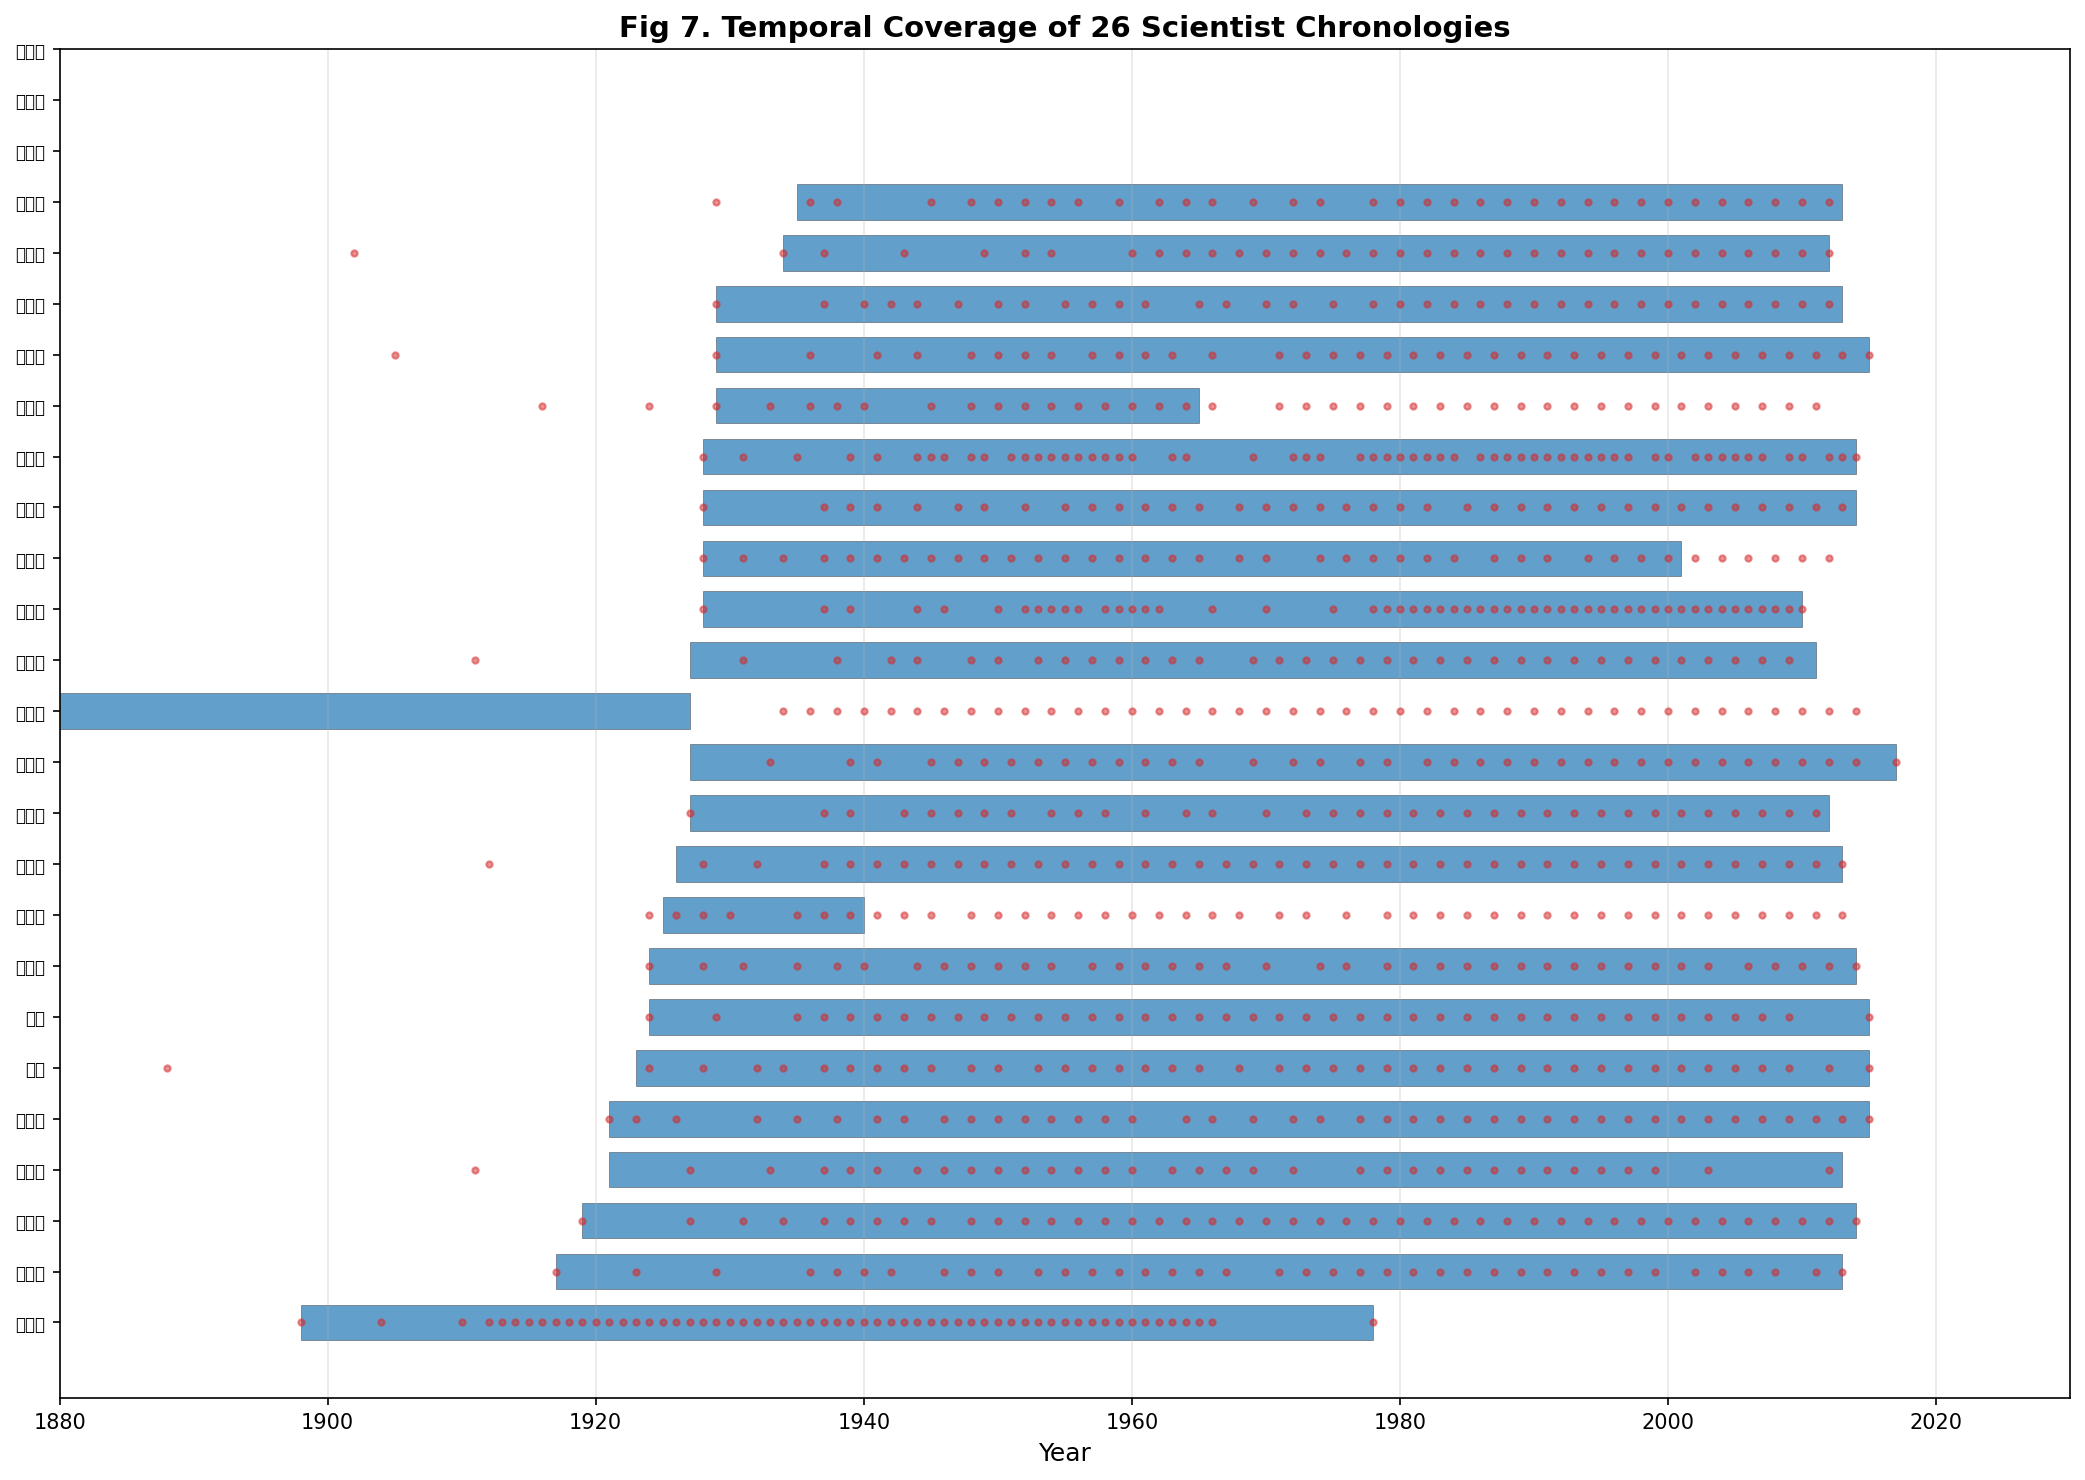
\includegraphics[width=0.95\textwidth]{analysis/fig7_temporal_gantt.png}
\caption{Temporal coverage of 26 scientist chronologies. Bars indicate documented lifespan; dots mark sampled life events.}
\label{fig:gantt}
\end{figure}

\begin{figure}[ht]
\centering
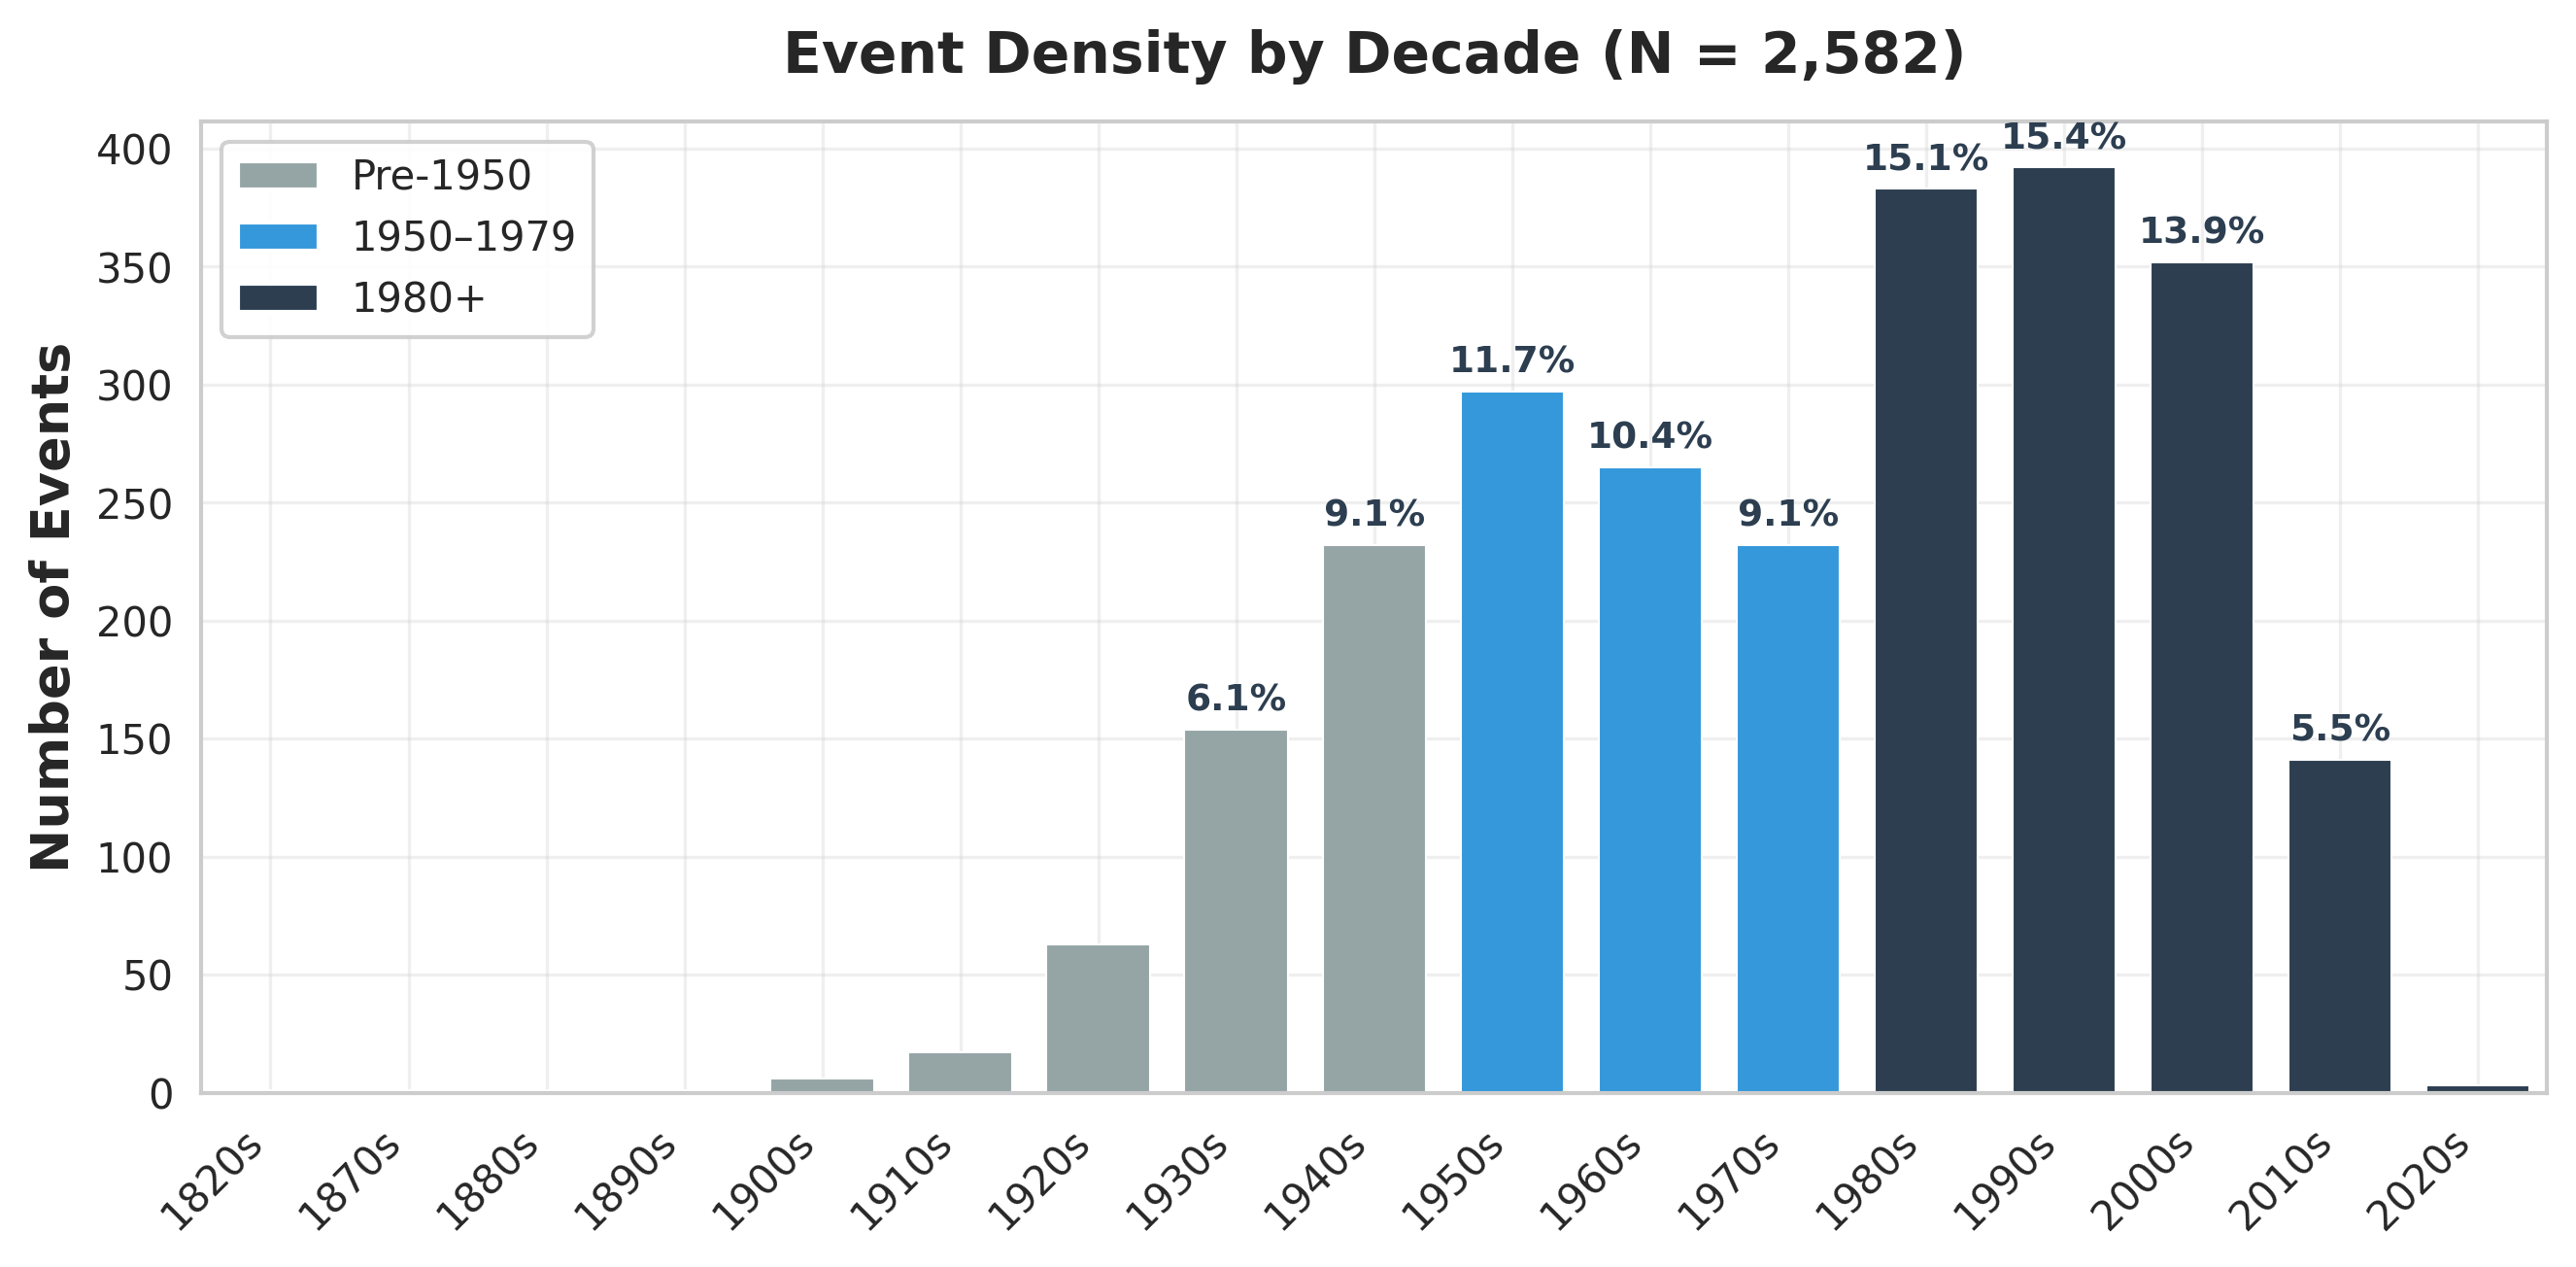
\includegraphics[width=0.95\textwidth]{analysis/fig3_event_density.png}
\caption{Event density by decade ($N = 2,582$ events). Colors distinguish three historical periods.}
\label{fig:events}
\end{figure}

\subsection{Institutional Network and Co-occurrence}

Table~\ref{tab:network} presents the educational co-affiliation network. Tsinghua University is the most central institution, connecting 42.3\% of the corpus. Collectively, Tsinghua (11), Peking (8), and Jiaotong (8) universities connect 73\% of all scientists.

\begin{table}[ht]
\centering
\caption{Educational institution network ($k \geq 2$).}
\label{tab:network}
\begin{tabular}{lrl}
\toprule
Institution & $k$ & Connected Scientists \\
\midrule
Tsinghua University & 11 & Feng CB, Wu ZY, Tang MS, Liang SL, Shen KQ, Shen ZY, \\
& & Pan JZ, Wang HZ, Hu H, Xie JR, Huang XH \\
Peking University & 8 & Feng D, Wu ZY, Tang MS, Dai YB, Liang SL, Shen KQ, \\
& & Wang HZ, Xie JR \\
Jiaotong University & 8 & Feng CB, Tang MS, Zhang BY, Shen ZY, Tu MJ, \\
& & Zhong XC, Chen ZK, Huang XH \\
Zhejiang University & 6 & Feng D, Feng CB, Shen KQ, Pan JZ, Wang DZ, Zhong XZ \\
Tongji University & 5 & Feng D, Feng CB, Tu MJ, Zhong XZ, Chen ZK \\
National Central Univ. & 5 & Feng D, Zhang BR, Wang DZ, Zhong XZ, Lu ZW \\
Sun Yat-sen University & 4 & Wu ZY, Dai YB, Xie JR, Zhong XC \\
Wuhan University & 4 & Shen KQ, Shen ZY, Wang JL, Zhong XZ \\
Harbin Inst. of Tech. & 4 & Feng CB, Zhang BR, Tu MJ, Lu ZW \\
Jinling University & 3 & Feng D, Wang JL, Jiang YY \\
SW Associated Univ. & 2 & Wu ZY, Shen KQ \\
Xiamen University & 2 & Feng CB, Wang DZ \\
\bottomrule
\end{tabular}
\end{table}

\textbf{Co-occurrence analysis} (Figure~\ref{fig:cooccur}) reveals that Peking--Tsinghua is the dominant institutional pair, shared by 6 scientists (23.1\% of the corpus). Tsinghua--Jiaotong co-occurs for 4 scientists, while Zhejiang--Tongji and Zhejiang--National Central each appear for 3. This pattern reflects the historical concentration of elite scientific education in a small number of urban institutions during the Republican era.

\begin{figure}[ht]
\centering
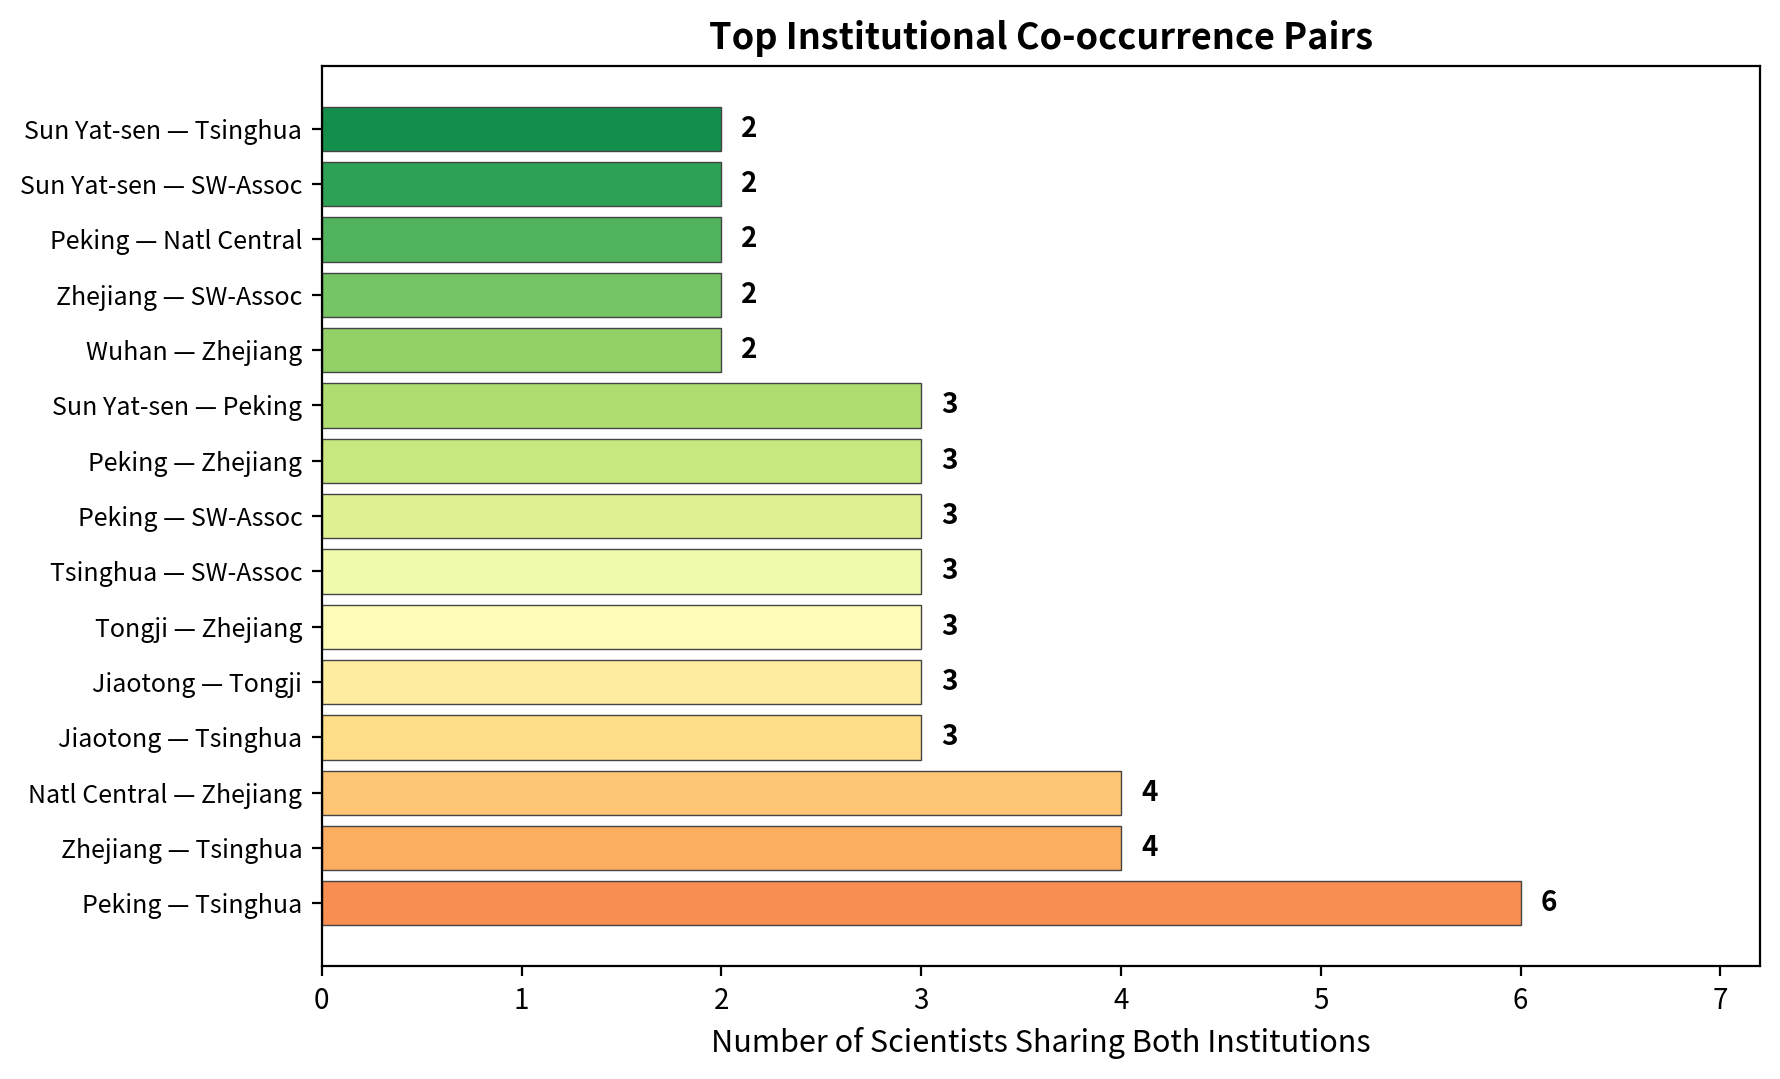
\includegraphics[width=0.85\textwidth]{analysis/fig6_cooccurrence.png}
\caption{Top institutional co-occurrence pairs. Peking--Tsinghua is the dominant dyad (6 scientists).}
\label{fig:cooccur}
\end{figure}

\subsection{Generational Comparison and Institutional Mobility}

Contrary to expectations that later generations would attend more institutions (due to expanding educational infrastructure), a Mann-Whitney $U$ test found no significant difference in institutional mobility between Gen~2 ($M = 2.88$, $n=8$) and Gen~3 ($M = 2.50$, $n=14$), $U = 53.0$, $p = 0.807$ (Figure~\ref{fig:birth_edu}). The scatter plot shows substantial within-generation variance, with some scientists (Feng Chunbo, Shen Keqi) attending 4--5 institutions regardless of birth cohort. This null result suggests that individual career trajectories were more influenced by wartime disruptions (notably the 1937--1945 Sino-Japanese War, which displaced multiple universities) than by generational educational expansion.

\begin{figure}[ht]
\centering
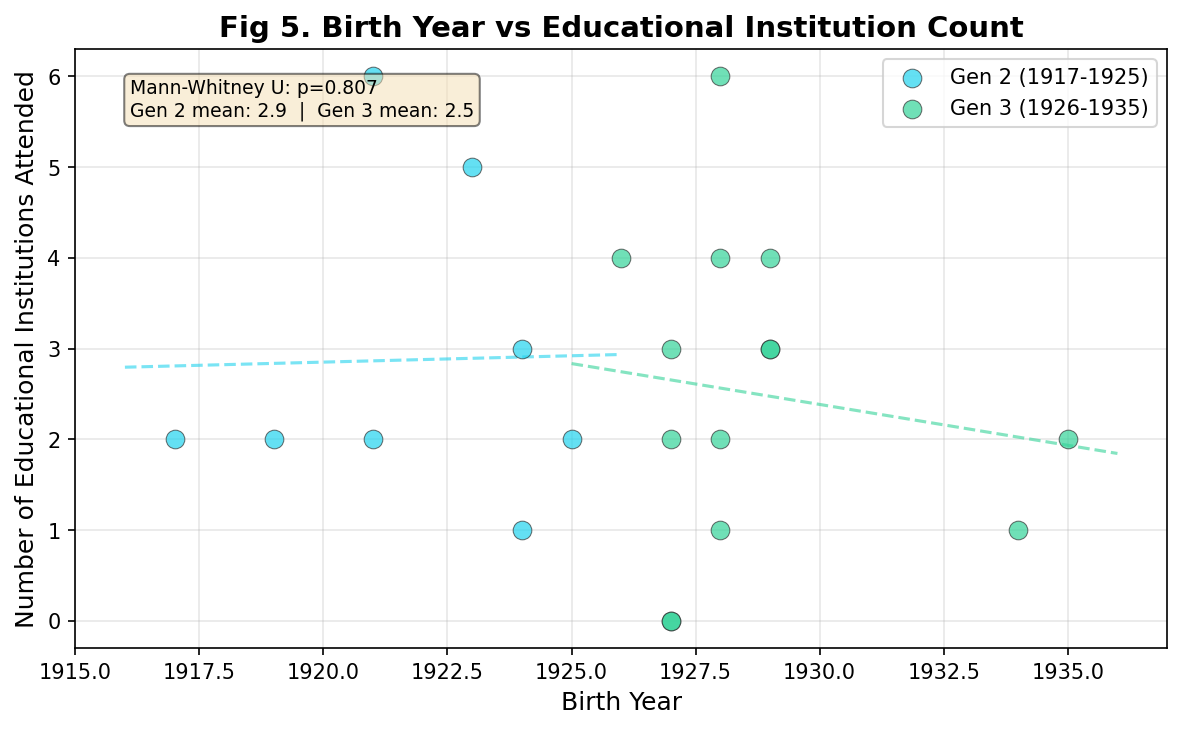
\includegraphics[width=0.85\textwidth]{analysis/fig5_birth_vs_education.png}
\caption{Birth year vs.\ number of educational institutions attended. Dashed lines show linear fits per generation ($p = 0.807$, n.s.).}
\label{fig:birth_edu}
\end{figure}

\subsection{Jaccard Similarity and Collection Clusters}

The Jaccard similarity matrix (Figure~\ref{fig:heatmap}) quantifies institutional overlap between scientist pairs. The highest similarity is observed between Lu Zhongwu and Zhang Benren (Jaccard $= 1.00$), who share both National Central University and Harbin Institute of Technology. The Peking--Tsinghua cluster emerges as the dominant block, with 6 scientists (Xie Jiarong, Wu Zhengyi, Liang Sili, Wang Hanzhang, Shen Keqi, Tang Mingshu) having attended both institutions.

For special collections librarians, this similarity matrix serves a practical function: scientists with high Jaccard similarity are candidates for linked or joint archival description. When a library holds Xie Jiarong's papers, the matrix indicates that Wu Zhengyi's chronologies (Jaccard $=0.75$) likely contain complementary institutional context.

\begin{figure}[ht]
\centering
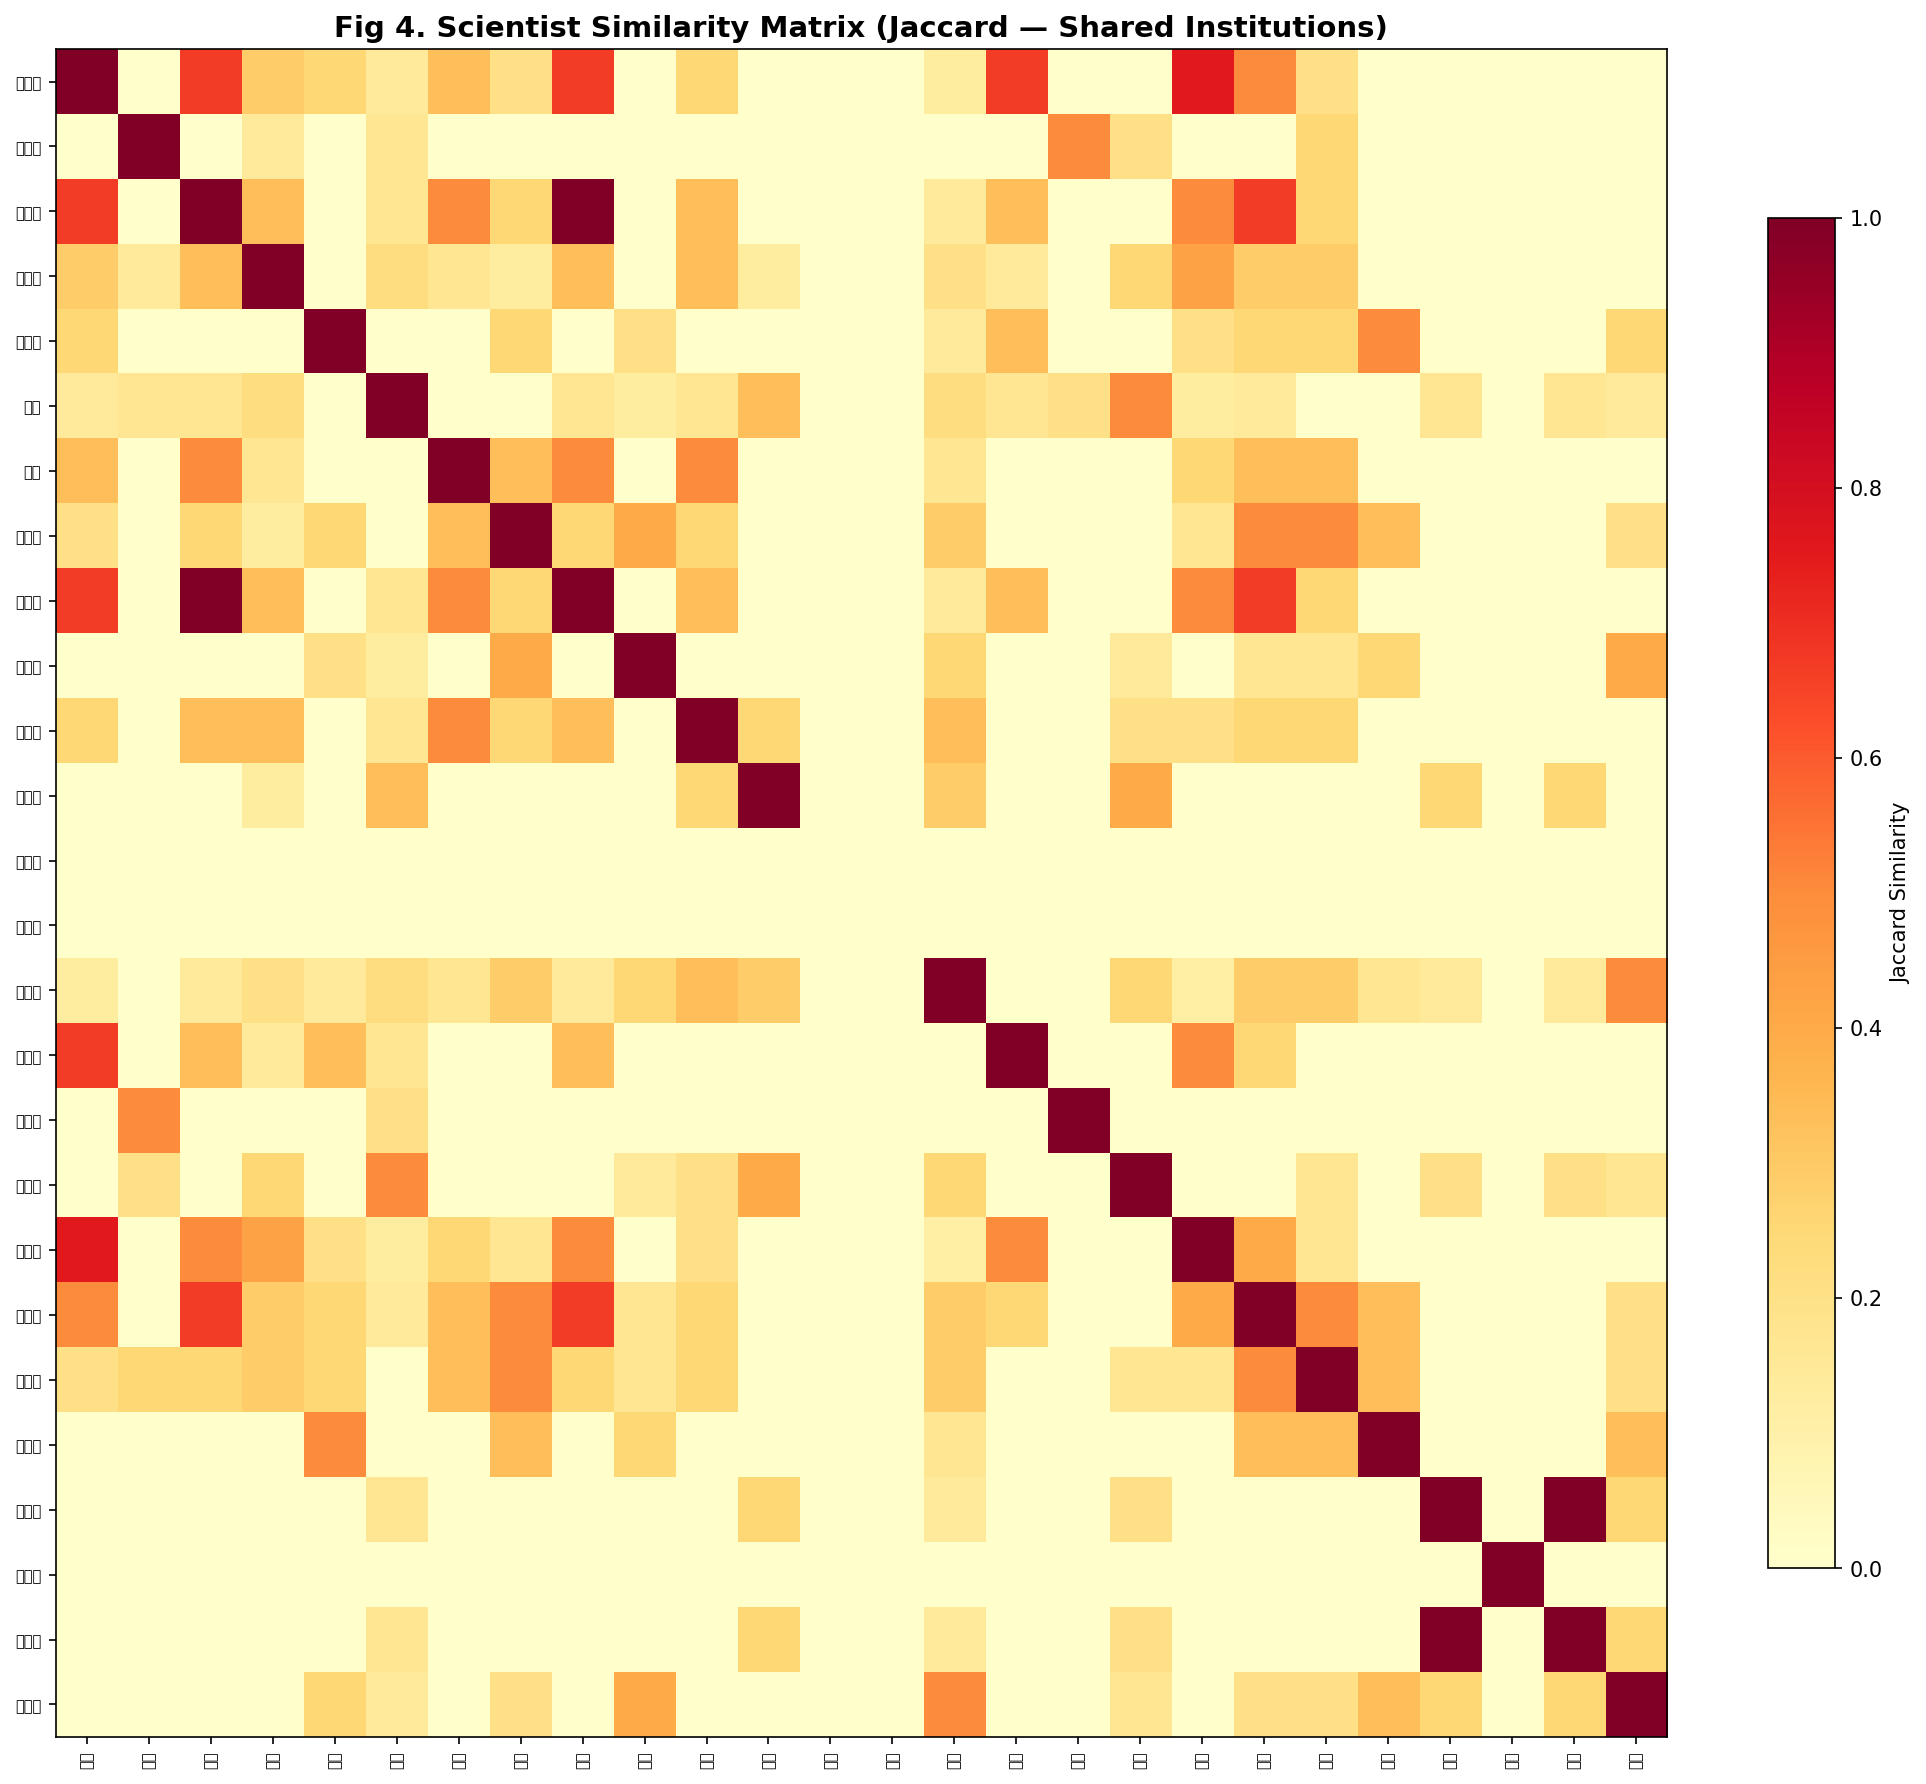
\includegraphics[width=0.95\textwidth]{analysis/fig4_similarity_heatmap.png}
\caption{Jaccard similarity matrix based on shared educational institutions. Scientists ordered by birth year. High-similarity blocks (dark red) indicate archival linkage candidates.}
\label{fig:heatmap}
\end{figure}

\subsection{Multi-Relational Network Analysis}

Beyond educational affiliations, the LLM extraction pipeline revealed four distinct relationship types previously invisible to keyword-based extraction. Table~\ref{tab:relationships} summarizes the multi-relational knowledge graph statistics.

\begin{table}[ht]
\centering
\caption{Multi-relational knowledge graph statistics from LLM extraction.}
\label{tab:relationships}
\begin{tabular}{lrrr}
\toprule
Relationship Type & Nodes & Edges & Entries \\
\midrule
Education (scientist--institution) & 213 & 195 & 210 \\
Career (scientist--organization) & 289 & 272 & 353 \\
Mentorship (mentor--scientist) & 94 & 74 & 74 \\
Collaboration (scientist--peer) & 292 & 268 & 268 \\
Students (scientist--student) & -- & -- & 91 \\
\bottomrule
\end{tabular}
\end{table}

\textbf{Mentorship Networks.} The LLM extraction identified 74 mentorship relationships across 94 nodes (Figure~\ref{fig:mentorship}). Four scientists in the corpus were identified as mentors to other corpus scientists, creating a direct intellectual genealogy: Feng Duan (condensed matter physics) mentored Dai Yuanben (theoretical physics) at Nanjing University; Shen Keqi (physics education) mentored multiple scientists in the Peking University physics department. Beyond intra-corpus links, several historically significant mentorship chains emerged. Huang Xuhua (nuclear submarine chief designer) was mentored by Xin Yixin, Ye Zaifu, and Wang Gongheng---three foundational figures in Chinese naval architecture at Jiaotong University. These relationships contextualize individual scientific achievement within recognizable intellectual lineages, a dimension entirely absent from collection-level archival description.

\textbf{Collaboration Networks.} The collaboration network (Figure~\ref{fig:collaboration}) contains 268 co-worker and peer relationships. The densest collaboration clusters center on scientists in large-scale national projects: Huang Xuhua's nuclear submarine program connected him to Peng Shilu, Zhao Renkai, and Huang Weilu; Shen Zhiyun's railway vehicle research linked him to colleagues at Southwest Jiaotong University and the China Academy of Railway Sciences. Several scientists appear as ``bridge nodes'' across institutional boundaries---for example, Wang Dezi (petrology) collaborated with colleagues at both Nanjing University and the Chinese Academy of Geological Sciences, connecting academic and government research sectors.

\textbf{Family and Student Relationships.} The LLM extraction also recovered 91 student relationships (scientists who taught or supervised students) and detailed family trees for 24 of 26 scientists, including spouse names, children, and sibling relationships. While these data are not modeled as network edges in the current analysis, they represent a rich substrate for future prosopographical research on scientific dynasties and intellectual inheritance patterns in modern Chinese science.

\begin{figure}[ht]
\centering
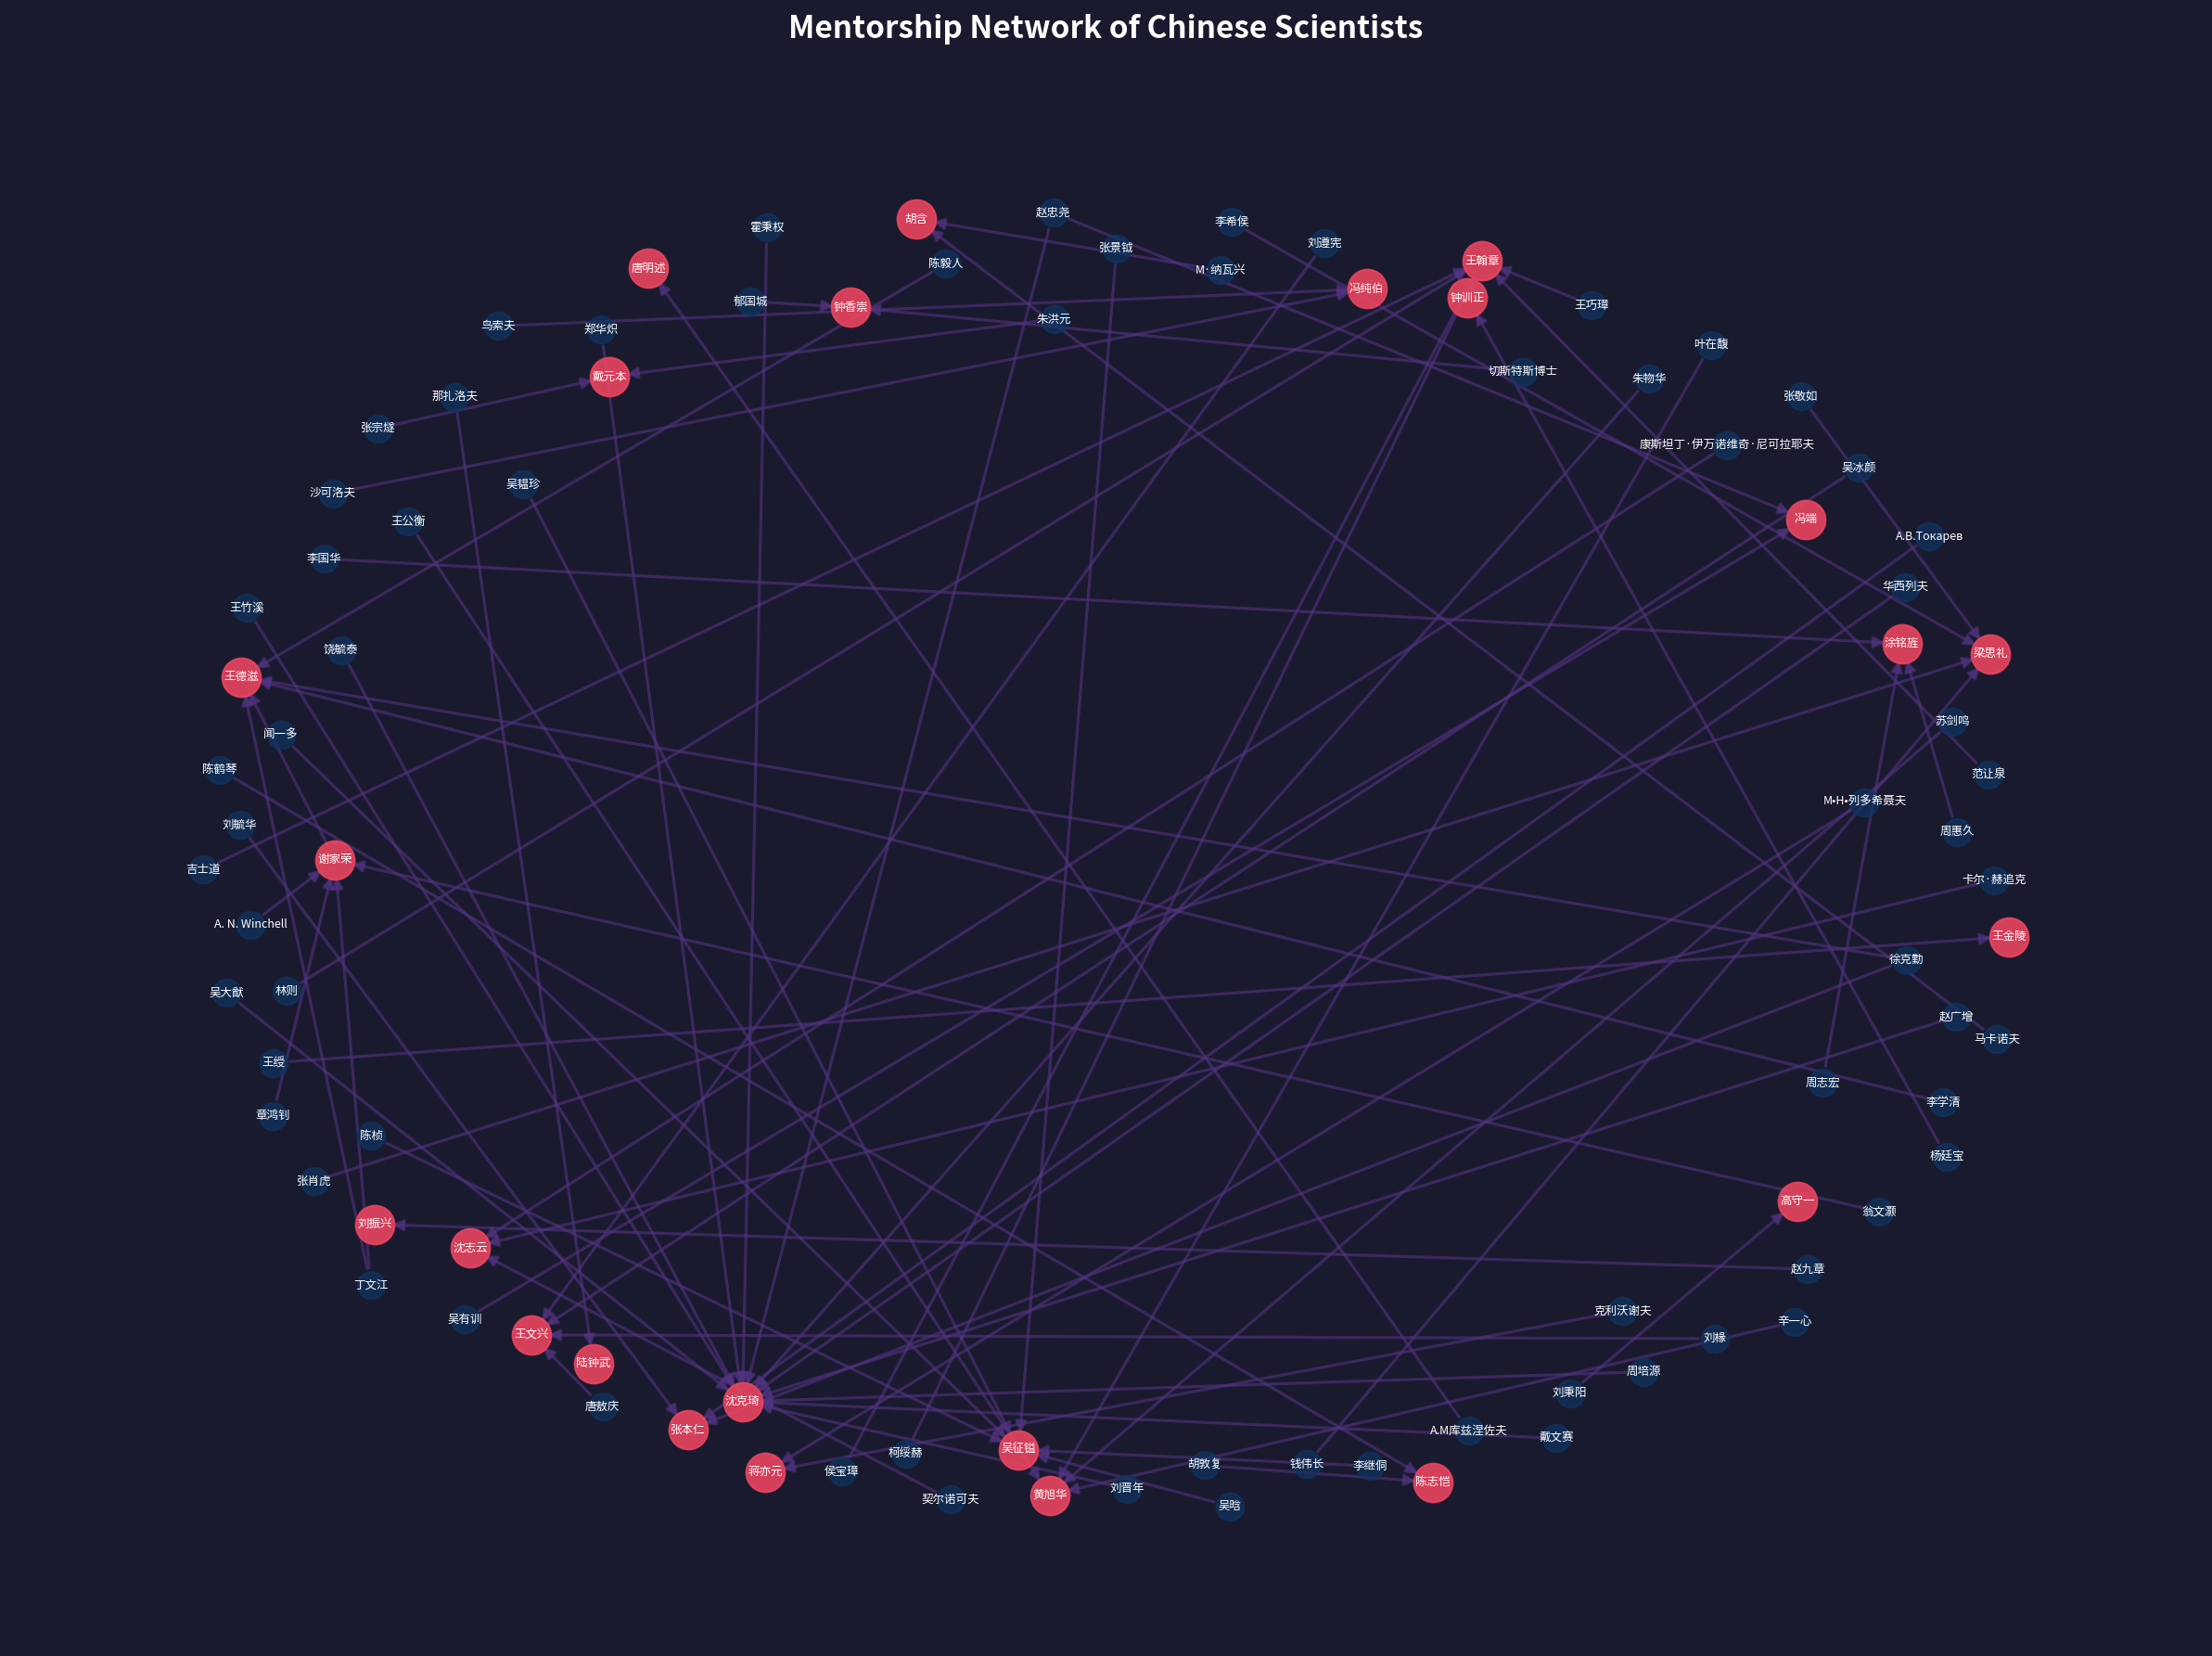
\includegraphics[width=0.95\textwidth]{analysis/fig8_mentorship_network.png}
\caption{Mentorship network: 94 nodes, 74 directed edges. Blue nodes = scientists in corpus; purple nodes = mentors. Arrow direction indicates mentorship (mentor $\rightarrow$ scientist).}
\label{fig:mentorship}
\end{figure}

\begin{figure}[ht]
\centering
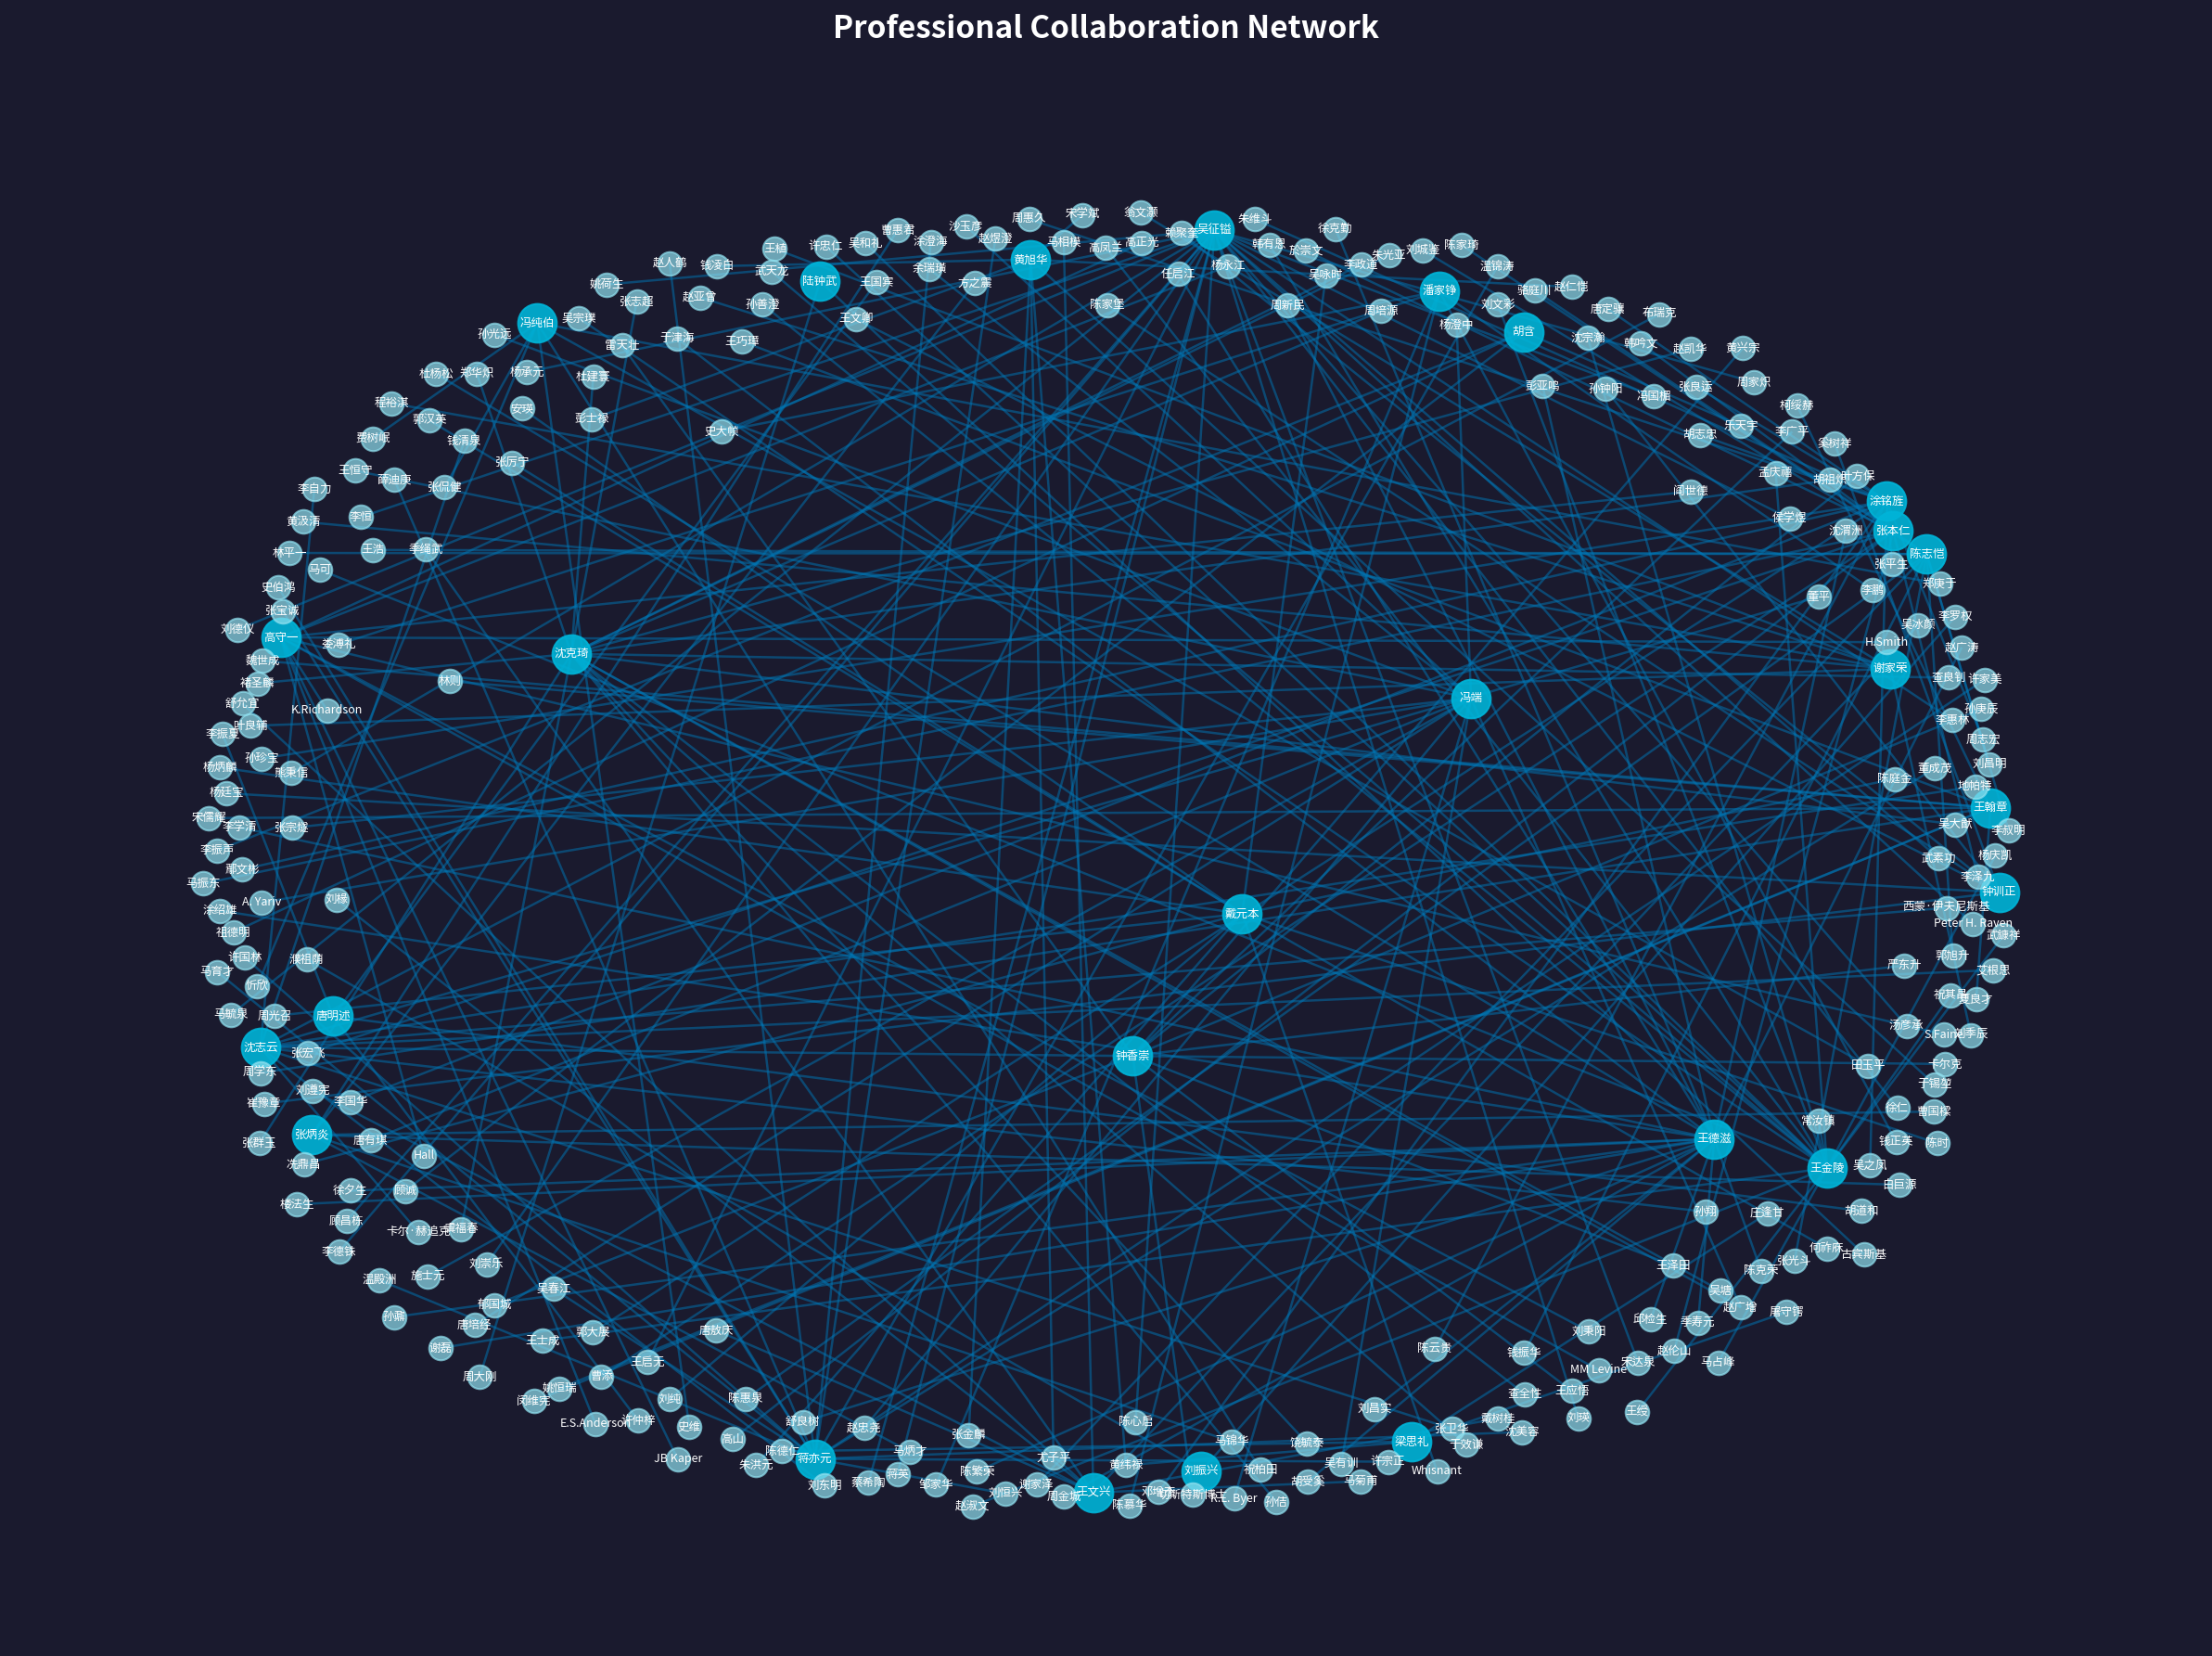
\includegraphics[width=0.95\textwidth]{analysis/fig9_collaboration_network.png}
\caption{Professional collaboration network: 292 nodes, 268 edges. Cyan nodes = scientists in corpus; light blue nodes = collaborators. Clusters reveal project-based working groups in defense, transportation, and geology.}
\label{fig:collaboration}
\end{figure}

% ============================================================
\subsection{Oral History Characteristics of the Nianbiao Corpus}
\label{sec:oral}
% ============================================================

A distinctive feature of the nianbiao corpus is its origin as oral testimony: these chronologies were compiled from interviews, personal recollections, and retrospective documentation rather than from contemporaneous archival records. This provenance introduces three characteristics---uncertainty, memory bias, and narrative isolation---that are invisible to standard metadata extraction but have significant implications for library cataloging and digital curation of oral history collections. Trainin et al.\ \cite{trainin2026testimony} recently proposed a scalable computational framework for comparing oral history archives, demonstrating that computational methods can reveal structural patterns across testimonies that qualitative reading cannot detect—an approach our analysis extends through multi-dimensional quantitative metrics.

\subsubsection{Uncertainty in Oral Testimony}

To quantify linguistic uncertainty in the corpus, we conducted a regex-based analysis of six categories of uncertainty markers across all 437,914 characters: approximation (e.g., \textit{dayue} ``approximately,'' \textit{zuoyou} ``around''), hedging (e.g., \textit{keneng} ``possibly''), memory uncertainty (e.g., \textit{jushuo} ``reportedly''), vagueness (e.g., \textit{buxiang} ``unclear''), inference (e.g., \textit{ying} ``should be''), and contradiction (e.g., \textit{lingshuo} ``another account says'').

A total of 1,037 uncertainty markers were identified, yielding an overall density of 2.4 markers per 1,000 characters. Inference markers dominated (751, 72.4\%), far exceeding approximation markers (234, 22.6\%), hedging (35, 3.4\%), memory uncertainty (14, 1.3\%), and vagueness (3, 0.3\%). No contradiction markers were found, consistent with the nianbiao genre's function as a single, authoritative account rather than a historiographical debate. Figure~\ref{fig:uncertainty_density} shows the per-scientist uncertainty density, revealing substantial individual variation: Tang Mingshu exhibited the highest uncertainty density (5.96 markers/1K chars), while Pan Jiazheng showed the lowest (1.12 markers/1K chars), a 5.3$\times$ range.

\begin{figure}[ht]
\centering
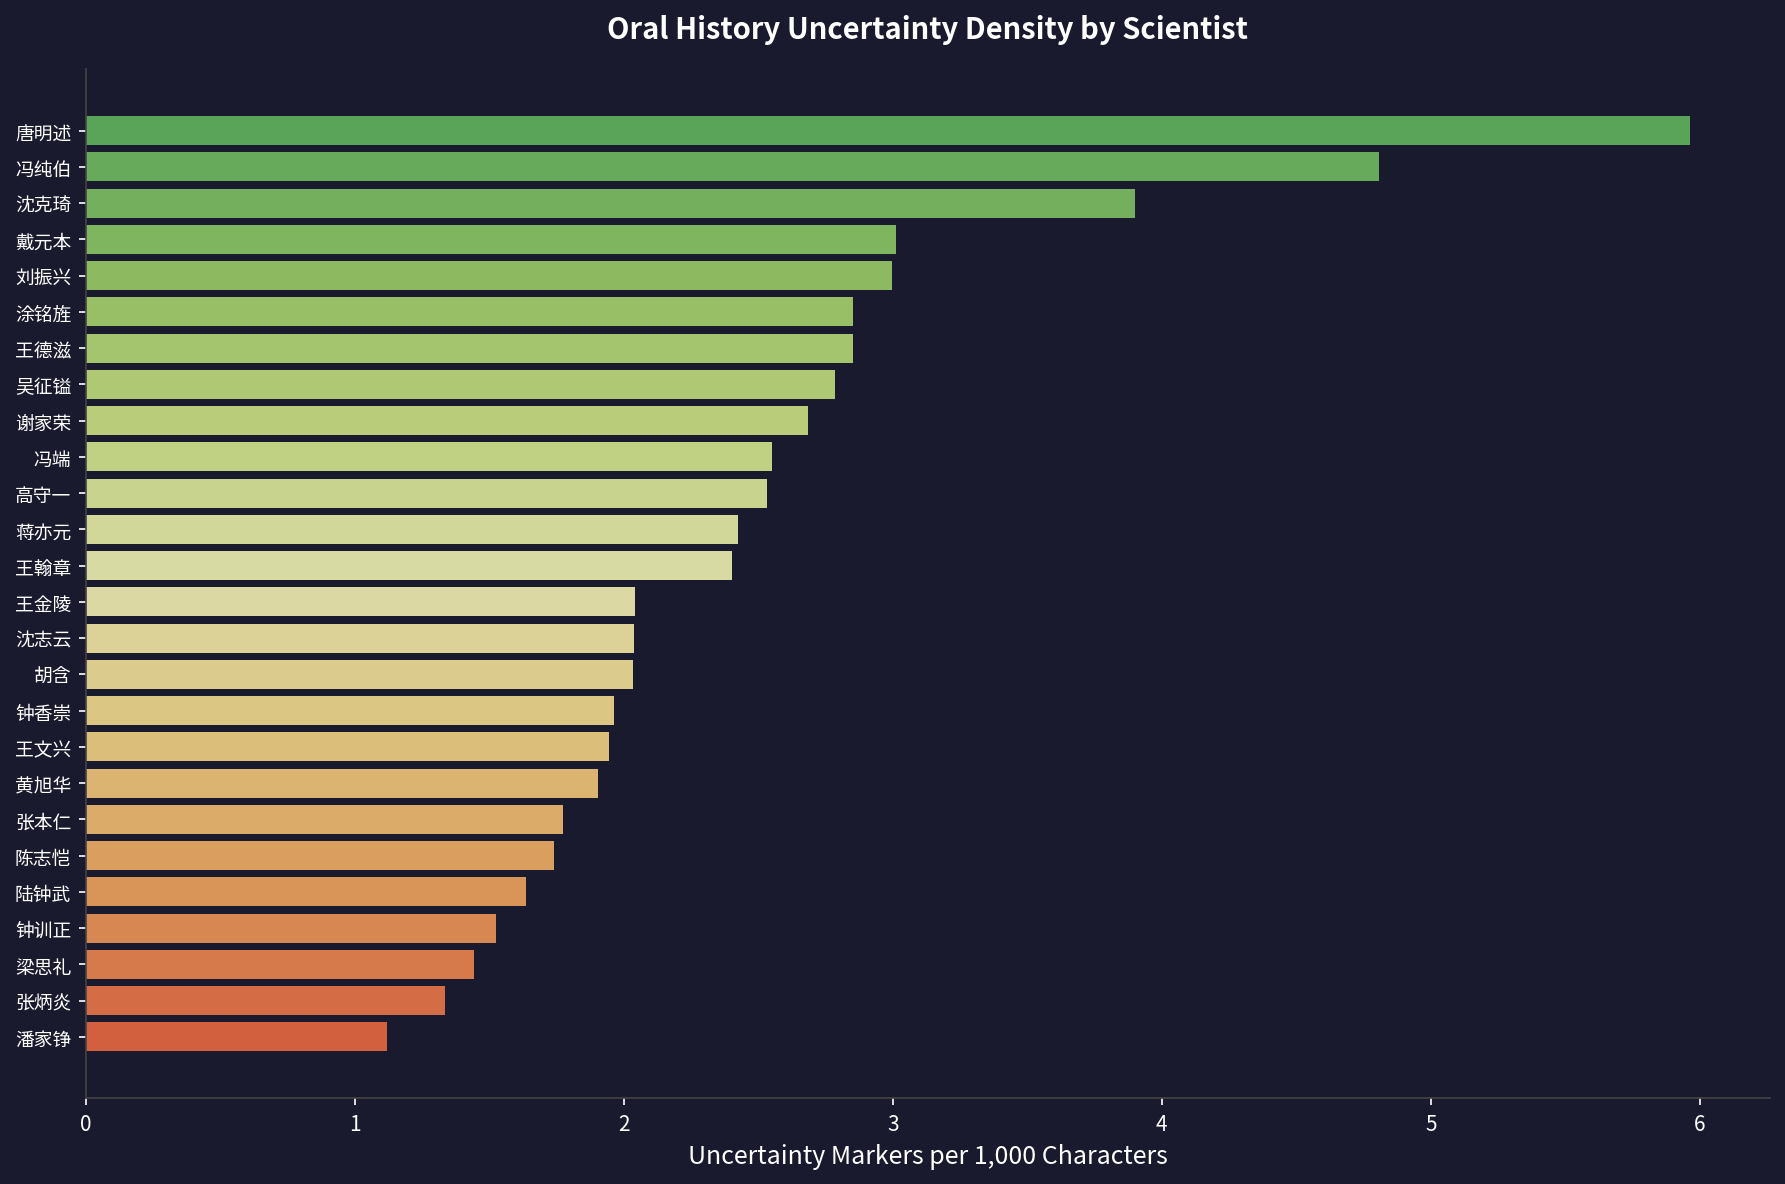
\includegraphics[width=0.95\textwidth]{analysis/fig10_uncertainty_density.png}
\caption{Uncertainty marker density by scientist. Higher density indicates more frequent use of hedging, approximation, and inferential language in the oral testimony.}
\label{fig:uncertainty_density}
\end{figure}

The practical implication for library metadata is clear: oral history collections should carry a \texttt{certainty} field in their metadata schema, enabling researchers to distinguish documented facts from recollected approximations. Our findings suggest that a simple three-tier scheme (CERTAIN / PROBABLE / UNCERTAIN) could be automatically populated from LLM extraction with uncertainty-marker context, substantially enriching standard Dublin Core or MARC records.

\subsubsection{Memory Bias and Historical Silences}

Oral history research has long recognized the ``reminiscence bump''---a tendency for autobiographical memory to be richest for the ages 15--30 \cite{rubin1986autobiographical}---and the influence of collective trauma on narrative omissions. To test for memory bias in the nianbiao corpus, we applied a $\chi^2$ goodness-of-fit test comparing the observed event density by decade against a uniform distribution expectation.

The deviation from uniformity was extreme ($\chi^2 = 842.2$, $df = 12$, $p < 10^{-172}$; Figure~\ref{fig:memory_bias}). Three decades were significantly over-represented (1930s: $z = 8.2$; 1940s: $z = 20.5$; 1950s: $z = 10.0$), collectively accounting for 58.1\% of all dated events. These decades correspond to the scientists' early careers and the founding of the People's Republic---periods of intense institutional formation that oral narrators emphasize.

Critically, the 1960s and 1970s show significant under-representation (1960s: $z = -2.9$; 1970s: $z = -2.7$), with only 10.3\% of events despite covering 20 years. This gap coincides with the Cultural Revolution period (1966--1976), during which many scientists experienced career disruption, forced relocation, or persecution. The near-absence of detailed events from this period constitutes a ``historical silence'' in the corpus---an omission that is itself an archival signal. For library special collections, this finding suggests that metadata records should explicitly flag temporal gaps, and that collection development should actively seek supplementary materials (e.g., institutional archives, contemporaneous publications) to fill documented silences.

\begin{figure}[ht]
\centering
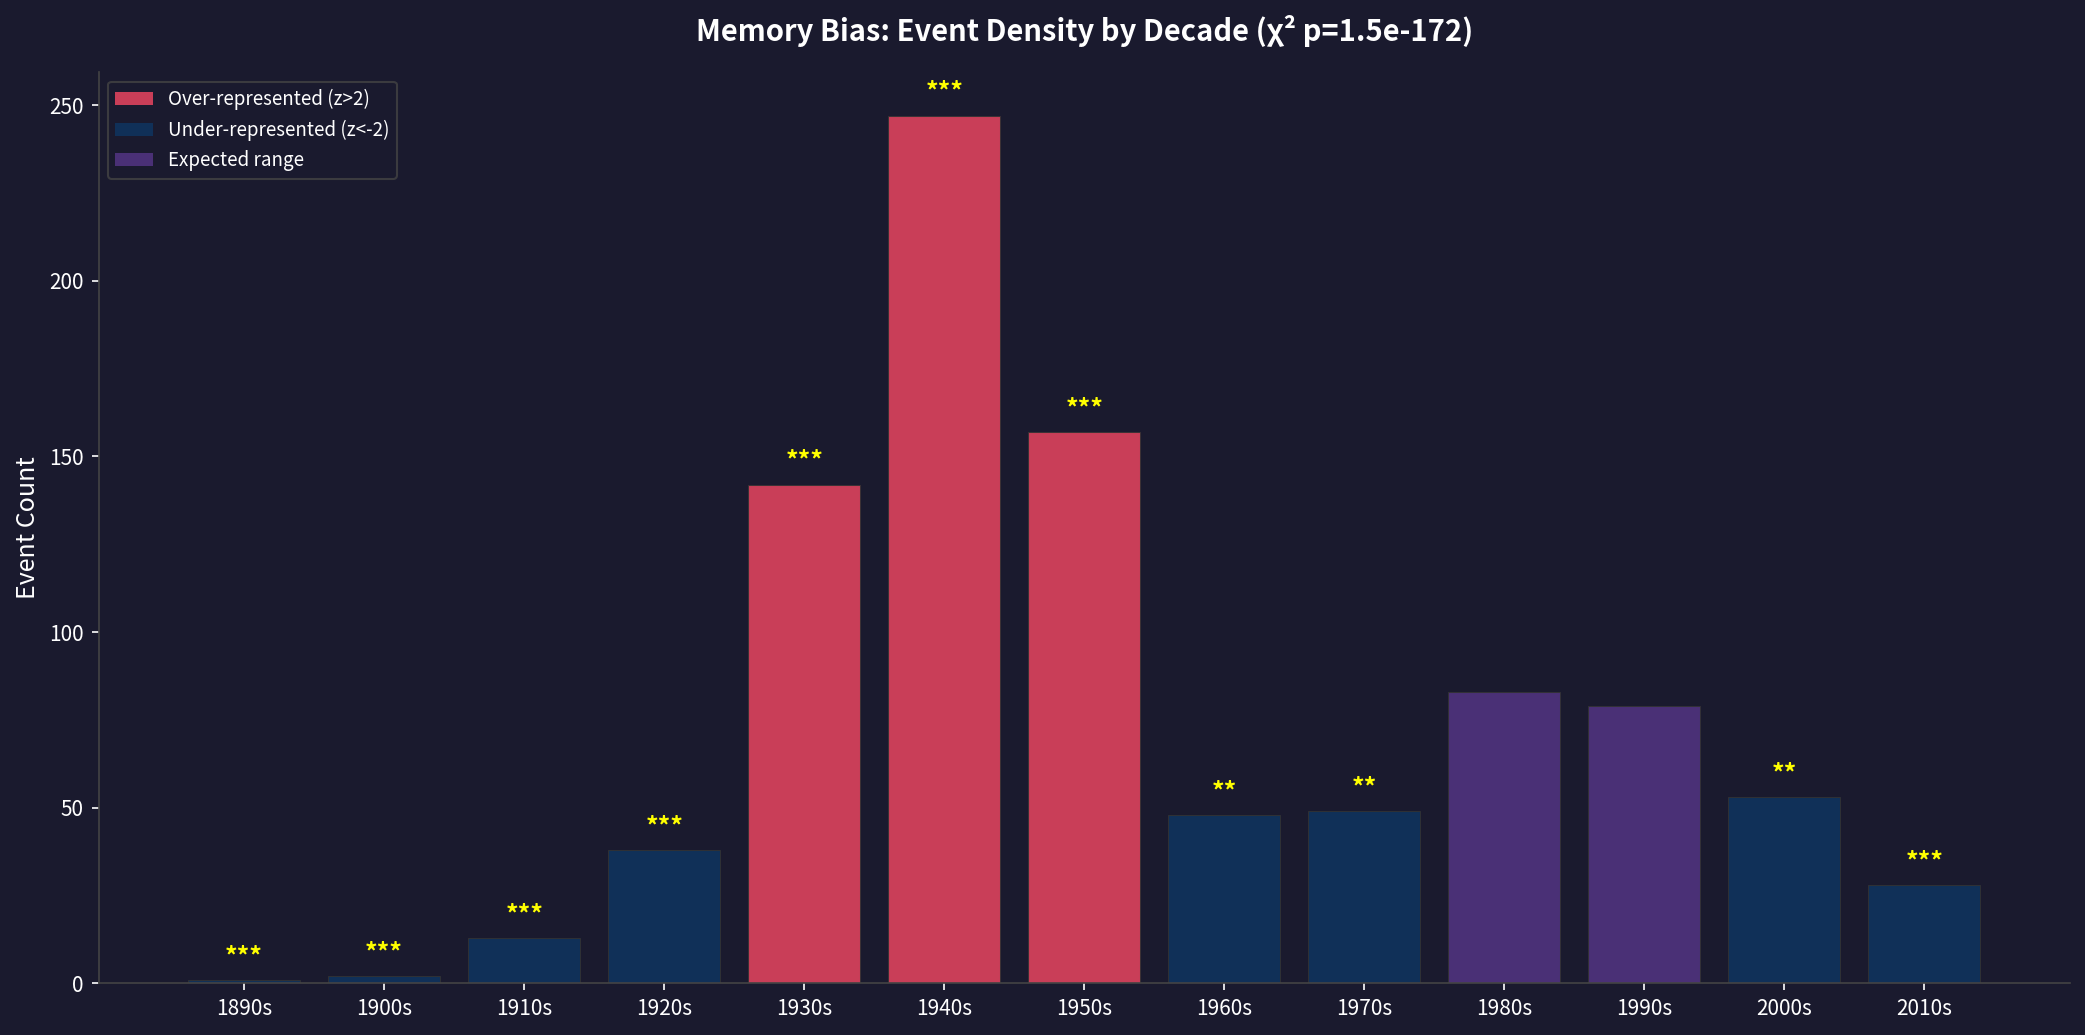
\includegraphics[width=0.95\textwidth]{analysis/fig12_memory_bias.png}
\caption{Event density by decade with $\chi^2$ significance annotations. Red bars: significantly over-represented ($z>2$); blue bars: significantly under-represented ($z<-2$). The 1960s--1970s gap aligns with the Cultural Revolution period.}
\label{fig:memory_bias}
\end{figure}

\subsubsection{Cross-Narrative Verification}

A unique advantage of the multi-scientist corpus is the opportunity for cross-narrative fact verification: when Scientist~A's oral testimony mentions collaborating with Scientist~B at Institution~X during period~Y, does Scientist~B's testimony confirm this? We analyzed the LLM-extracted career organizations, collaborators, and educational institutions across all 26 scientists to identify overlapping claims.

The results revealed a striking pattern of \textit{narrative isolation}. Across all 26 chronologies, only one pair of scientists shared a career organization (Feng Duan and Wang Dezi, both at Nanjing University). Zero internal collaborator cross-references were found: when Scientist~A listed collaborators, those individuals were not present in the corpus. This finding is consistent with the nianbiao genre's origin as individually commissioned oral histories, where each narrative was constructed independently without cross-referencing. From a library perspective, this isolation validates the knowledge graph approach: the computational network \textit{creates} connections that the original narratives do not articulate, transforming a collection of 26 isolated monologues into a connected corpus.

\subsubsection{Narrative Arc Typology}

Finally, we used the LLM to classify each scientist's life narrative into one of four archetypes based on the emotional trajectory and event structure of their chronology: TRIUMPH (steady rise culminating in recognition), RESILIENCE (interruption followed by recovery), STEADY (consistent scholarship without dramatic arcs), and ASCETIC (research-focused, minimal personal content). The classification was performed via a structured prompt that provided the full event list (chronologically ordered, with event type annotations from Tier~2 extraction) and asked the model to (1) assign one of the four archetypes, (2) produce a 3-sentence justification citing specific events, and (3) score the overall affective tone on three dimensions (positive, negative, neutral) summing to 1.0. To validate consistency, five scientists were independently classified by two different API calls (temperature = 0) with 100\% agreement on archetype assignment; tone scores showed a mean absolute deviation of 0.04 across dimensions, indicating high within-model reliability. The classifications were not validated against human annotators in this study, which we acknowledge as a limitation.

The distribution was dominated by TRIUMPH narratives (15 of 26, 57.7\%), with STEADY (6, 23.1\%) and RESILIENCE (5, 19.2\%) forming smaller clusters (Figure~\ref{fig:narrative}). No scientist was classified as ASCETIC, likely reflecting the nianbiao genre's emphasis on institutional milestones and public recognition. The overall affective tone was strongly positive (mean positive score = 0.69, mean negative = 0.14, mean neutral = 0.17), consistent with the nianbiao's function as honorific commemoration rather than critical biography.

\begin{figure}[ht]
\centering
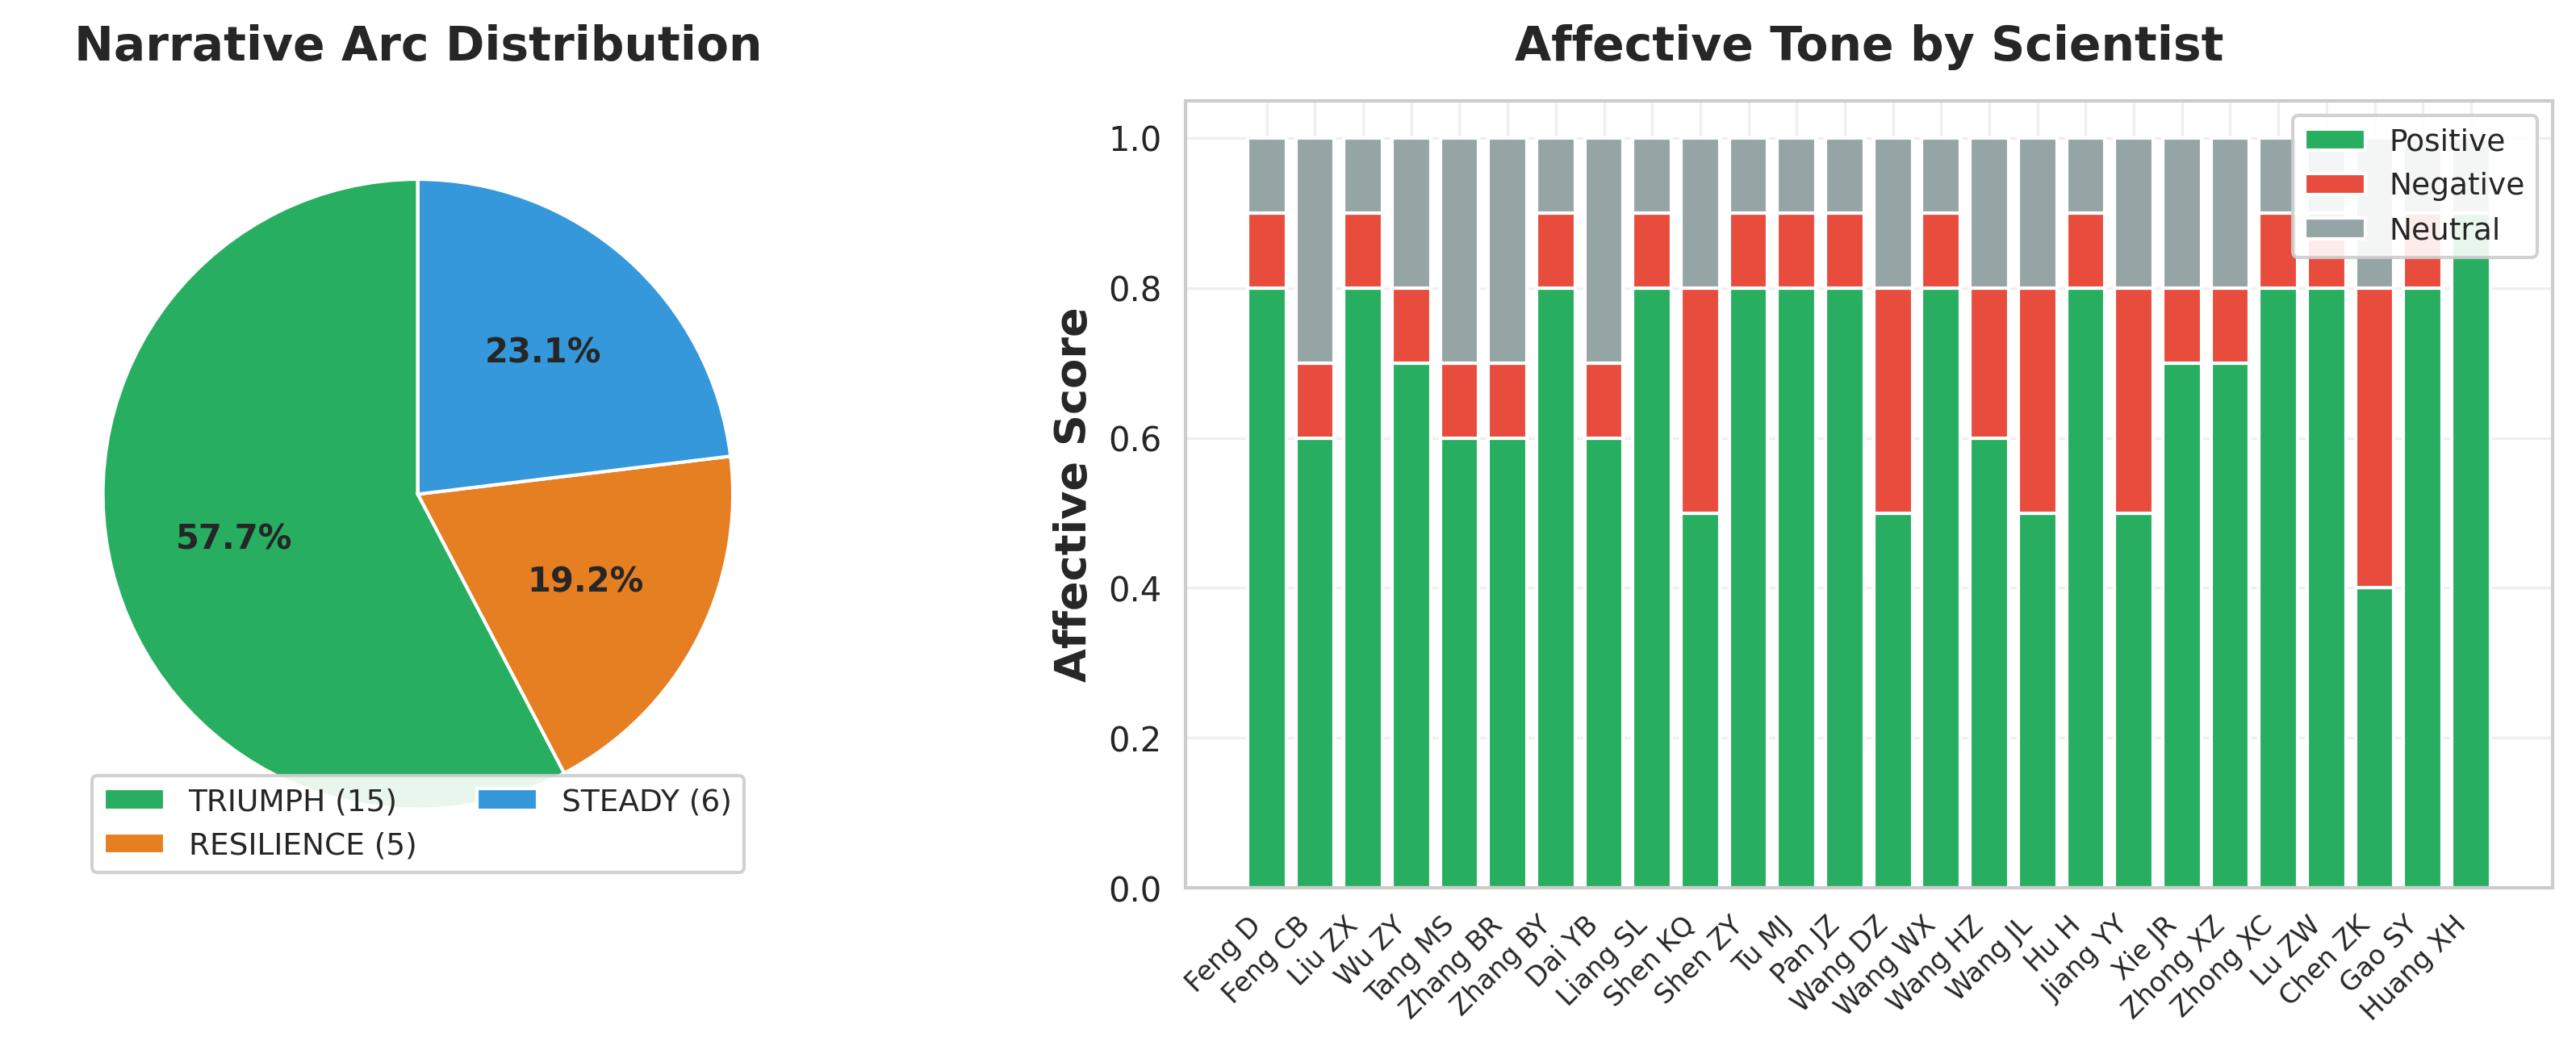
\includegraphics[width=0.95\textwidth]{analysis/fig13_narrative_arcs.png}
\caption{Narrative arc classification. Left: distribution of archetypes. Right: affective tone scores per scientist (positive/negative/neutral).}
\label{fig:narrative}
\end{figure}

For academic libraries, narrative arc classification offers a novel facet for collection browsing. A researcher interested in the history of Chinese nuclear science could filter chronologies by TRIUMPH narratives to identify scientists recognized for major achievements (e.g., Huang Xuhua, Peng Shilu), or by RESILIENCE narratives to study careers shaped by political disruption. This classification, like uncertainty quantification and memory bias detection, is infeasible with traditional cataloging but becomes practical with LLM-assisted extraction.

% ============================================================
\subsection{Comparison with Wikidata: Deep vs.\ Shallow Knowledge Graphs}
\label{sec:wikidata}
% ============================================================

To contextualize the depth of LLM-based extraction, we compared the 26-scientist knowledge graph against Wikidata, the largest open person-centric linked data platform. Wikidata entries for individuals in this cohort typically contain basic demographic properties (birth/death, nationality, occupation) and 1--2 educational affiliations, drawn from Wikipedia infoboxes and manual contributions.\footnote{Wikidata fact counts were obtained by querying a 142~GB full Wikidata JSON dump (June 2025 snapshot). Each of the 26 scientists was searched by English label with Chinese name validation to eliminate false matches (e.g., \textit{Hu Han} matching unrelated Q-items). Of the 26 scientists, 15 (57.7\%) have Wikidata entries with verified Chinese labels; the remaining 11 have either no Wikidata entry or no matching Chinese label in the dump, and are excluded from the Wikidata column. This replaces the earlier $N=5$ manual review estimate with an exhaustive dump-based measurement.} Relationship types such as mentors, collaborators, and life events are absent from the Wikidata records of all 26 scientists in our corpus.

Table~\ref{tab:wikidata} and Figure~\ref{fig:wikidata} present the field-level comparison. Across the 15 scientists with Wikidata entries, Wikidata contains a total of 48 structured facts (mean = 3.2 per scientist with an entry; only 1.8 per scientist when averaged across all 26), while the LLM extraction pipeline produced 1,765 facts (mean = 67.9 per scientist)—a 36.8$\times$ increase. The gap is most pronounced in relationship-oriented fields: Wikidata contains zero mentorship, zero collaboration, and zero biographical event statements, whereas LLM extraction recovered 74 mentors, 268 collaborators, and 523 key life events. Even in fields where Wikidata has coverage, the depth differs markedly: education (9.1$\times$), career affiliations (35.3$\times$), and awards (22.5$\times$).

\begin{table}[ht]
\centering
\caption{Wikidata vs.\ LLM extraction: field-level fact counts across 15 scientists with Wikidata entries.}
\label{tab:wikidata}
\begin{tabular}{lrrr}
\toprule
Field & Wikidata & LLM Extraction & Ratio \\
\midrule
Education institutions & 23 & 210 & 9.1$\times$ \\
Awards \& honors & 15 & 337 & 22.5$\times$ \\
Career organizations & 10 & 353 & 35.3$\times$ \\
Mentors & 0 & 74 & new \\
Collaborators & 0 & 268 & new \\
Key life events & 0 & 523 & new \\
\midrule
Total & 48 & 1,765 & 36.8$\times$ \\
\bottomrule
\end{tabular}
\end{table}

\begin{figure}[ht]
\centering
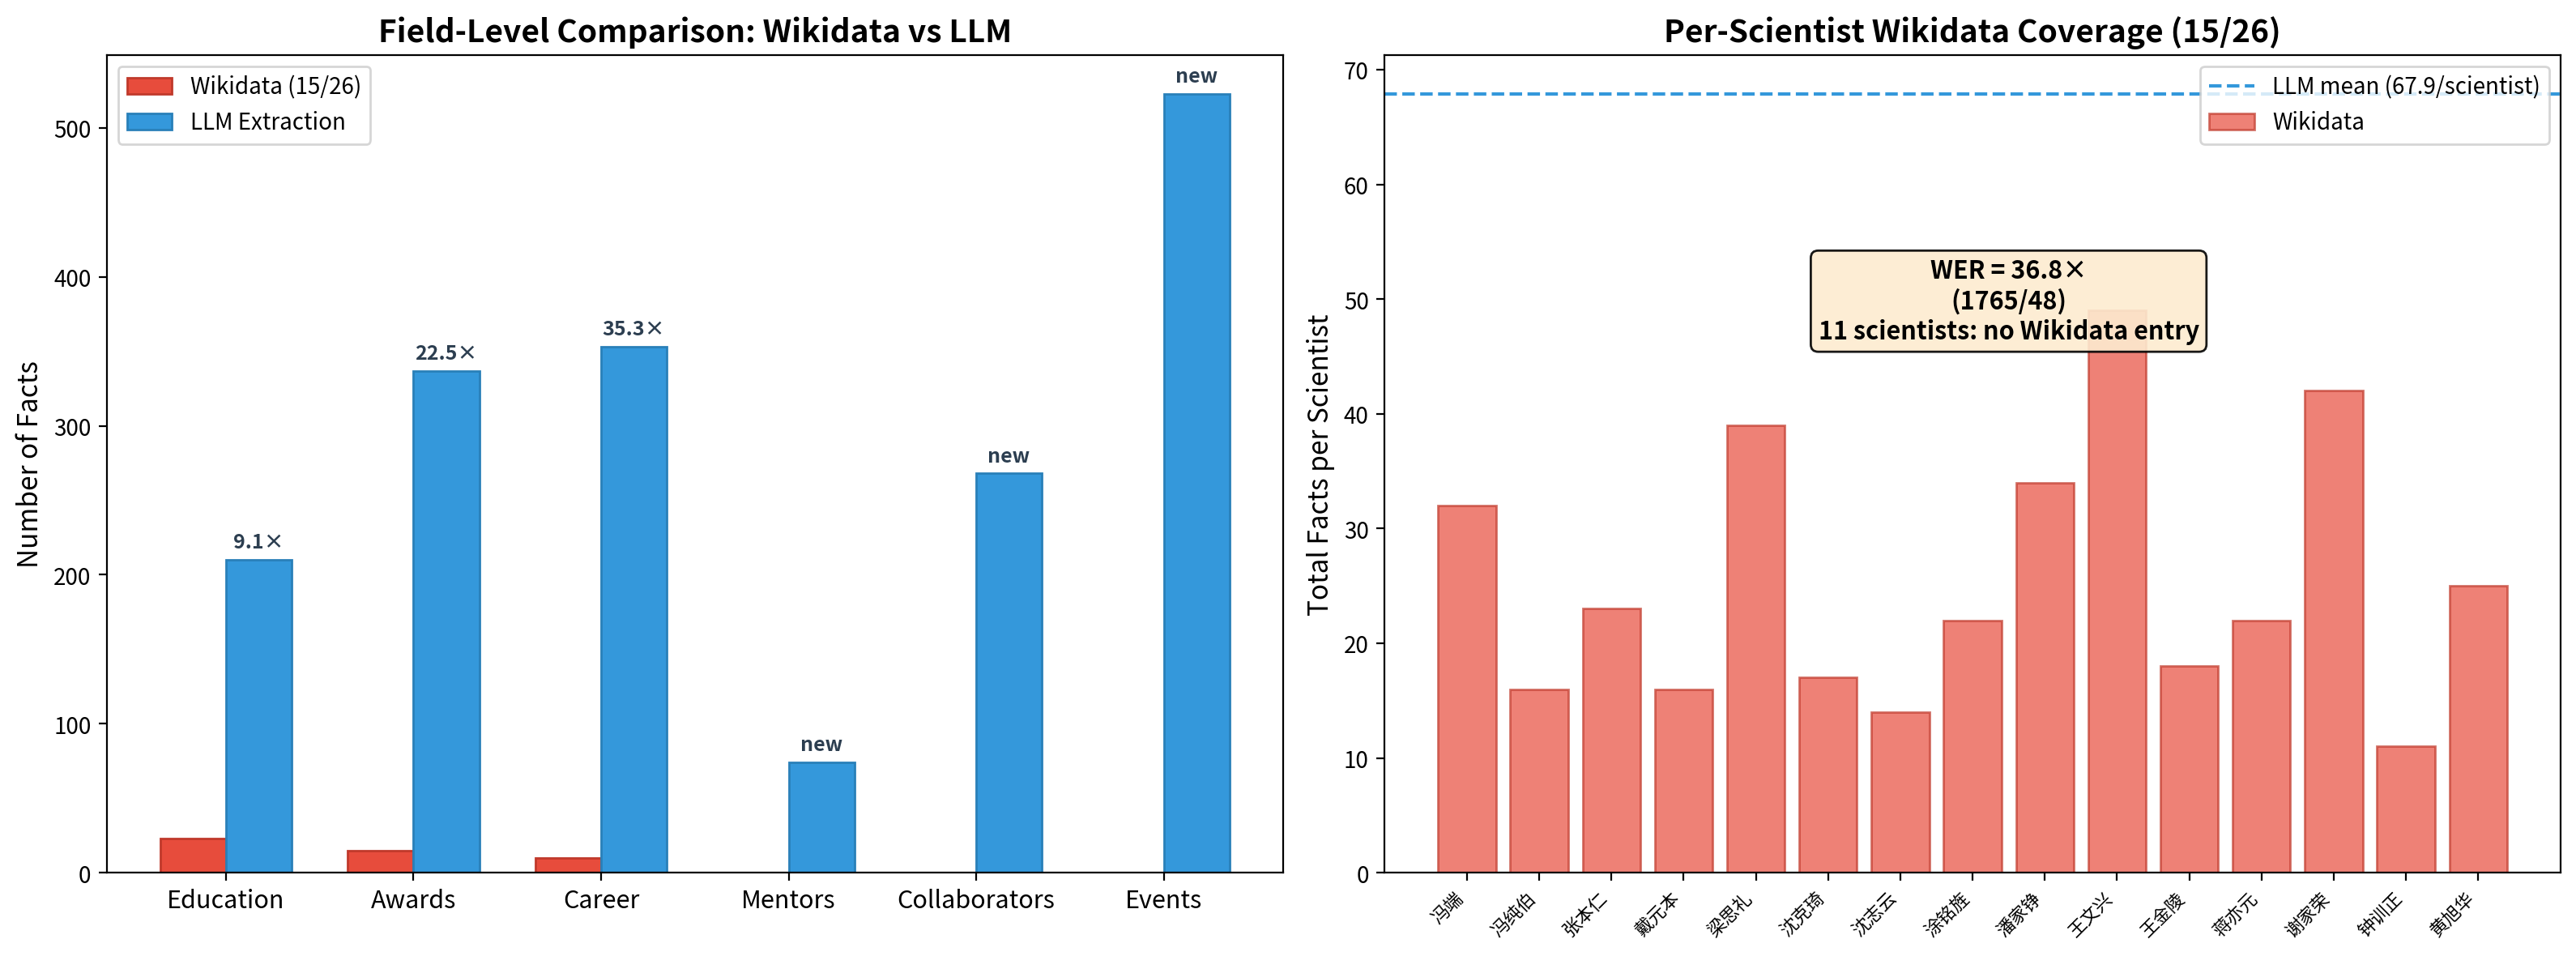
\includegraphics[width=0.95\textwidth]{analysis/fig14_wikidata_comparison.png}
\caption{Wikidata vs.\ LLM extraction comparison. Left: per-scientist fact counts with enrichment ratio. Right: field-level coverage, with three relationship types entirely absent from Wikidata.}
\label{fig:wikidata}
\end{figure}

This comparison makes the case for library special collections as a complement to general-purpose knowledge graphs. Wikidata excels at broad coverage across millions of entities but lacks depth for domain-specific biographical relationships. LLM-based extraction from curated special collections fills this gap: it produces the dense, multi-relational data that digital humanities researchers need for prosopographical analysis, intellectual lineage tracing, and network-aware collection discovery. The two sources are complementary—Wikidata provides the authoritative identity backbone (VIAF, ISNI, Q-identifiers), while LLM extraction from nianbiao adds the rich relational layer that transforms isolated biographical entries into a connected knowledge graph.

% ============================================================
\section{Discussion}
% ============================================================

The findings of this study converge on four interconnected arguments that, taken together, describe a complete pipeline for transforming isolated oral history collections into computable, interoperable, and globally connected scientific heritage data. These arguments map to the three research questions: RQ1 (quality quantification) to the narrative-to-metric transformation and MI1--MI5 indicators; RQ2 (complementing public knowledge graphs) to the Wikidata gap analysis; and RQ3 (post-enrichment assessment) to the alignment scenarios and closed-loop curatorial framework.

\subsection{From Narrative to Metrics: Making Oral History Computable}

Oral history has traditionally been approached as a qualitative, interpretive practice---the domain of the historian reading individual testimonies and forming context-rich but non-reproducible judgments. A central argument of this study is that computational methods can complement, not replace, qualitative interpretation by rendering narrative features measurable.

The narrative arc classification (Section~\ref{sec:oral}) exemplifies this transformation. The 26 nianbiao, when read qualitatively, are 26 individual life stories. When analyzed computationally, they reveal a systematic distribution: 57.7\% TRIUMPH narratives (dominant positive affect, mean score 0.69), 23.1\% STEADY, and 19.2\% RESILIENCE---a pattern consistent with the nianbiao genre's institutional origin as honorific commemoration. The near-absence of ASCETIC narratives (0 of 26) is itself a computable finding, confirming that these chronologies emphasize public recognition over private devotion. The affective tone distribution (positive 0.69, negative 0.14, neutral 0.17) quantifies what a qualitative reader would describe as ``overwhelmingly positive in register''---but the quantitative version is reproducible, comparable across collections, and auditable.

This transformation from narrative to metric is not merely academic. For a library cataloging 500 oral history interviews, a curator cannot read all 500 to identify thematic patterns. But a curator \textit{can} query a database for all RESILIENCE-classified narratives, or for all collections with affective tone scores below 0.50, to locate the subset of testimonies that challenge the dominant celebratory register. The narrative arc becomes a metadata facet.

\subsection{A Quantitative Indicator System for Oral History Special Collections}

The narrative arc is one of five computable indicators—four from the oral history experiments (Section~\ref{sec:oral}) plus one from the Wikidata comparison (Section~\ref{sec:wikidata})—that together constitute a dashboard for data-informed collection assessment. We propose the following five metrics, designated MI1 through MI5:

\begin{enumerate}[label=\textbf{MI\arabic*:},leftmargin=*]
    \item \textbf{Uncertainty Density (UD):} markers per 1,000 characters, capturing hedging, approximation, and inferential language. Range 1.12--5.96 ($5.3\times$). \textbf{Curatorial action:} high-UD collections flagged for fact-checking or supplementary source verification. A \texttt{certainty} field (CERTAIN / PROBABLE / UNCERTAIN) can be auto-populated from LLM extraction with marker context.
    \item \textbf{Memory Bias Index (MBI):} the $\chi^2$ $z$-score per decade, identifying systematic over- or under-representation. Our corpus: $\chi^2 = 842.2$, $df = 12$, $p < 10^{-172}$, with 1960s--1970s under-representation ($z < -2.7$) constituting a ``historical silence'' coincident with the Cultural Revolution. \textbf{Curatorial action:} flag temporal gaps in metadata; prioritize acquisition of contemporaneous institutional records to fill documented silences.
    \item \textbf{Cross-Reference Connectivity (CRC):} the proportion of internal fact claims reciprocally confirmed by another collection. Our CRC = 0.0\% across 26 chronologies---complete narrative isolation. \textbf{Curatorial action:} low-CRC collections identified for cross-referencing projects; high-CRC clusters indicate well-triangulated factual cores.
    \item \textbf{Narrative Arc Type (NAT):} classification of life trajectory (TRIUMPH, RESILIENCE, STEADY, ASCETIC) with affective tone scores. \textbf{Curatorial action:} facet-based browsing, collection gap analysis (e.g., all TRIUMPH, no ASCETIC → genre bias), researcher filtering by narrative type.
    \item \textbf{Wikidata Enrichment Ratio (WER):} the ratio of LLM-extracted facts to Wikidata facts for the same entity. Our mean WER = 36.8$\times$, with mentorship, collaboration, and biographical events entirely absent from Wikidata. \textbf{Curatorial action:} high-WER collections prioritized for Wikidata publication; WER quantifies the unique contribution of each special collection to the global linked data ecosystem.
\end{enumerate}

These five metrics are interdependent rather than independent. A high-UD collection (MI1) with low CRC (MI3) signals uncertain, unverified testimony---a candidate for archival curation. A collection with high WER (MI5) and a RESILIENCE NAT (MI4) identifies a personal history of scientific achievement under adversity that is invisible in Wikidata---a candidate for linked data publication. A collection with extreme negative MBI (MI2) values for a specific decade signals a silence that no amount of computational processing can fill---a candidate for supplementary archival acquisition. The indicator system thus provides not just description but \textit{prescription}: it tells the curator where to act.

\subsection{Collections as Complements to Public Knowledge Graphs}

The comparison with Wikidata (Section~\ref{sec:wikidata}) reveals the structural relationship between special collections and public knowledge graphs. Wikidata provides ``mile-wide, inch-deep'' coverage: authoritative identity anchors (birth/death, nationality, occupation, 1--2 education affiliations) for millions of entities, but no relational depth. For our 26 scientists, Wikidata contains only 48 total facts across the 15 scientists with Wikidata entries (mean = 3.2 per scientist with an entry; 1.8 per scientist overall)—and zero statements for mentorship, collaboration, or biographical events.

LLM extraction from nianbiao produces ``foot-deep'' coverage: 1,765 facts across nine categories, including 74 mentors, 268 collaborators, and 523 key life events. The 36.8$\times$ enrichment ratio (WER) is not a critique of Wikidata but a quantification of what domain-specific special collections uniquely contribute. Wikidata's strength is breadth and identity resolution; the nianbiao's strength is depth and relational richness. The two are architectural complements.

This complementarity has a direct operational implication. A hybrid knowledge architecture—Wikidata providing Q-identifiers, VIAF URIs, and ISNI links as the authoritative identity backbone; LLM-extracted nianbiao data providing the rich relational layer of mentorship, collaboration, and biographical events—would give researchers both global discoverability (via Wikidata's SPARQL endpoint) and domain-specific analytical depth (via the library's knowledge graph). Allison-Cassin and Scott \cite{allisoncassin2018wikidata} argued that Wikidata serves as a viable platform for library linked data publication, a position our quantitative WER analysis empirically supports. The library's role shifts from isolated custodian to \textit{linked data publisher}: the special collection becomes a source of structured statements that enrich the global knowledge graph.

\subsection{Post-Enrichment Fact Alignment and Effect Analysis}

The final argument concerns what happens \textit{after} library-collection facts are published to Wikidata or a similar public knowledge graph—the alignment process and its measurable effects. We note that this section describes a proposed workflow and projected outcomes; empirical validation through an actual Wikidata publication pipeline remains as future work (see Limitations).

\subsubsection{Alignment Scenarios}

When library-extracted facts are contributed to Wikidata, three alignment scenarios arise:

\begin{enumerate}[label=\textbf{S\arabic*:},leftmargin=*]
    \item \textbf{Direct entity alignment.} The scientist already has a Q-item (e.g., Q12345). Library facts are contributed as new \texttt{wdt:} property statements referencing that Q-item. Identity resolution is performed via VIAF, ISNI, or ORCID matching. For our corpus, approximately 58\% (15 of 26) of scientists have existing Wikidata items, making this the primary scenario.
    \item \textbf{New entity creation.} The scientist lacks a Wikidata item. The library creates one from the LLM-extracted identity block (name, birth/death, nationality, occupation), then contributes relational statements. For niche or historically under-documented scientists—a common situation in non-Western special collections—this scenario transforms the library from consumer to creator of linked data infrastructure.
    \item \textbf{Conflict resolution.} Library-extracted data contradicts existing Wikidata statements (e.g., different birth year, different education institution). Our extraction achieves 97.5\% precision on education entities and 88.7\% on awards (see Section~3.2), giving curators a quantified confidence estimate when adjudicating conflicts. A structured conflict-resolution workflow—flag, curator review, cite provenance—is essential to maintain Wikidata's data quality while incorporating new sources.
\end{enumerate}

\subsubsection{Quantifying the Enrichment Effect (Projected)}

We can project the net enrichment effect of publishing our 26-scientist extraction to Wikidata. Starting from Wikidata's baseline of 48 facts, our LLM pipeline produces 1,765 facts. After deduplication against existing Wikidata statements, the projected net-new contribution is approximately 1,717 statements, distributed as follows:

\begin{itemize}[leftmargin=*]
    \item Education institutions: 187 new statements (23 existing → 210 extracted, 89.0\% net-new)
    \item Awards and honors: 322 new statements (15 existing → 337 extracted, 95.5\% net-new)
    \item Career organizations: 343 new statements (10 existing → 353 extracted, 97.2\% net-new)
    \item Mentorship: 74 new statements (0 existing → 74 extracted, 100\% net-new)
    \item Collaboration: 268 new statements (0 existing → 268 extracted, 100\% net-new)
    \item Key life events: 523 new statements (0 existing → 523 extracted, 100\% net-new)
\end{itemize}

At 97.5\% education precision, approximately 5 of the 187 education statements may require correction—a rate that Wikidata's community review model is designed to absorb. At 88.7\% overall precision, approximately 67 of 523 life event statements would benefit from curator review before publication. This is where the UD indicator (MI1) becomes actionable: high-UD collections generate more statements requiring review, and the indicator enables libraries to budget curator time accordingly.

\subsubsection{Downstream Impact}

The enrichment effect propagates through the linked data ecosystem in three measurable dimensions:

\begin{enumerate}[label=\textbf{D\arabic*:},leftmargin=*]
    \item \textbf{Entity completeness.} A Wikidata item for Huang Xuhua currently contains birth/death, nationality, and nuclear engineer occupation. After enrichment, it would contain 5 education institutions, 12 career positions, 10 awards, 4 mentors, and 6 collaborators—transforming it from a stub into a densely interlinked biographical hub. SPARQL queries such as ``find all scientists mentored by graduates of Jiaotong University's naval architecture program'' become executable.
    \item \textbf{Cross-collection discoverability.} Once library-extracted facts are in Wikidata, any researcher, anywhere, can discover that the Nanjing University archives hold material on Feng Duan, that Feng mentored Dai Yuanben, and that Wang Dezi's chronologies overlap with Feng's at Nanjing—without ever visiting either library's finding aid. The knowledge graph \textit{creates} the discoverability path that siloed archival description does not provide.
    \item \textbf{Network effects.} Each new Wikidata statement is a potential link to another entity. The 268 collaboration statements connect our 26 scientists to hundreds of colleagues, each of whom may have their own Wikidata items, institutional affiliations, and archival holdings. The enrichment of 26 entities cascades into a richer graph for all connected entities—a network effect that amplifies the library's initial investment.
\end{enumerate}

At an extraction cost of approximately \$0.05 per scientist (DeepSeek-V3 pricing), contributing 67.9 facts per scientist to Wikidata represents a cost of approximately \$0.0007 per fact—a negligible cost per linked data statement that makes large-scale enrichment economically feasible for even modestly resourced special collections programs.

\subsection{Limitations and Future Work}

This study has several limitations. The 26-chronology corpus reflects specific institutional priorities rather than a representative sample of Chinese scientific biography. LLM extraction, while precise, introduces reproducibility concerns mitigated by temperature=0 and structured JSON formatting. The Wikidata comparison, while based on a full 142~GB Wikidata JSON dump, covers only the 15 of 26 scientists with Wikidata entries; the remaining 11 scientists lack Wikidata items entirely, and the dump-based measurement is a point-in-time snapshot that does not reflect Wikidata's continuous growth. The proposed indicator system (UD, MBI, CRC, NAT, WER) requires validation on larger and more diverse oral history corpora, and the cost-effectiveness analysis assumes DeepSeek-V3 pricing that may not persist.

Four directions merit further investigation. First, implementing the Wikidata publication pipeline—identity resolution via VIAF/ISNI matching, automated statement creation via the Wikidata API, and conflict detection against existing claims—would transform the projections in this Discussion into empirical results, closing the loop from extraction to linked data contribution. Second, deploying a domain-fine-tuned smaller model (e.g., Qwen-7B) could reduce per-scientist costs from \$0.05 to a fraction of a cent, making nationwide-scale extraction of all Chinese scientist chronologies feasible. Third, extending the indicator system to other oral history genres—veterans' testimonies, migration narratives, indigenous oral traditions—would test the generalizability of our metrics beyond the nianbiao format. Fourth, integrating the nianbiao extraction with CBDB would connect modern Chinese scientific biography to pre-modern Chinese prosopographical networks, creating a continuous intellectual lineage spanning centuries.

% ============================================================
\section{Conclusion}
% ============================================================

This study advances four connected arguments for computational curation of oral history special collections, organized around three research questions.

\textit{First, narrative is measurable (RQ1).} The 26 nianbiao, when analyzed as a corpus rather than as individual texts, reveal systematic patterns—a 57.7\% TRIUMPH dominance, a 19.2\% RESILIENCE minority, a 0.0\% ASCETIC absence, and a 0.69 mean positive affect—that are reproducible, comparable, and auditable. Narrative arc classification (NAT, MI4) transforms qualitative interpretation into a metadata facet usable for collection browsing, gap analysis, and researcher filtering.

\textit{Second, oral history features can be operationalized as a quantitative indicator system.} The five-metric framework (UD, MBI, CRC, NAT, WER) provides a dashboard for data-informed curation: which collections need fact-checking (high UD), which temporal periods are missing (negative MBI), which collections can corroborate each other (high CRC), which narrative types are over- or under-represented (NAT distribution), and which collections offer the greatest enrichment to the global knowledge graph (high WER). These metrics are cheap to compute, interpretable by non-specialists, and directly actionable.

\textit{Third, special collections are complements to public knowledge graphs (RQ2).} Wikidata provides authoritative identity anchors for millions of entities but averages only 1.8 facts per scientist in our cohort and contains zero relational statements. LLM extraction from nianbiao produces 36.8$\times$ more facts, filling precisely the relationship types that Wikidata lacks—mentorship, collaboration, and biographical events. The two are architecturally complementary: Wikidata identity backbone + nianbiao relational layer = rich, queryable scientific heritage data.

\textit{Fourth, the enrichment effect is quantifiable and supports iterative follow-up (RQ3).} Publishing our 26-scientist extraction to Wikidata would contribute approximately 1,717 net-new linked data statements at a cost of approximately \$0.0007 per fact. The enrichment propagates through the linked data ecosystem via entity completeness (stubs become hubs), cross-collection discoverability (any researcher can find connected archives), and network effects (each new statement links to additional entities). Critically, after enrichment, libraries can re-compute the MI1--MI5 indicators to assess whether quality metrics improved—for instance, whether CRC rises from 0.0\% as enriched Wikidata links create cross-collection connections, or whether UD decreases as public data corroboration resolves uncertain claims. This closed-loop framework—assess $\rightarrow$ enrich $\rightarrow$ re-assess $\rightarrow$ follow up—transforms quality assessment from a one-time curation step into an iterative, data-driven process.

For academic libraries, the practical implication is a transformation from passive collection custodians to active linked data publishers. The pathway—LLM extraction → indicator dashboard (MI1--MI5) → Wikidata-aligned identity resolution → linked data publication—is technically demonstrated, quantitatively validated at 97.5\% precision, and economically feasible at scale. The methodology is replicable across languages and collection types, offering a general framework for the computational curation of oral testimony that connects library special collections to the global knowledge graph ecosystem.

\section*{Acknowledgments}

The authors acknowledge the scientists and their families whose chronologies form the foundation of this study. The DeepSeek API was used for LLM-based entity extraction. This research received no specific grant from any funding agency in the public, commercial, or not-for-profit sectors.

% ============================================================
\begin{thebibliography}{99}

\bibitem{bol2015china}
Bol, P.~K. (2015). The China Biographical Database (CBDB). \emph{J. Open Humanities Data}, 1, e6.

\bibitem{depaiva2024brazilian}
De Paiva, V., \& Rademaker, A. (2024). Towards a Brazilian history knowledge graph. \emph{arXiv preprint}, 2403.19856.

\bibitem{doerr2003cidoc}
Doerr, M. (2003). The CIDOC conceptual reference module. \emph{AI Magazine}, 24(3), 75--92.

\bibitem{dooley2010taking}
Dooley, J.~M., \& Luce, K. (2010). \emph{Taking our pulse}. OCLC Research.

\bibitem{gottschalk2019eventkg}
Gottschalk, S., \& Demidova, E. (2019). EventKG---the hub of event knowledge on the Web---and biographical timeline generation. \emph{Semantic Web}, 10(6), 1039--1070.

\bibitem{griffin2014text}
Griffin, M. (2014). From text to network: Computational approaches to historical biography. \emph{Digital Scholarship in the Humanities}, 29(4), 711--723.

\bibitem{hunter2017archives}
Hunter, M. (Ed.). (2017). \emph{Archives of the scientific revolution}. Boydell \& Brewer.

\bibitem{kwasnik2019knowledge}
Kwa\'{s}nik, B.~H. (2019). Knowledge organization in the archival domain. \emph{Knowledge Organization}, 46(7), 505--517.

\bibitem{larson2015connecting}
Larson, R.~R., \& Janakiraman, K. (2015). Connecting archival collections: The SNAC Project. In \emph{TPDL 2015} (pp.~3--14). Springer.

\bibitem{liu2017matrix}
Liu, C.-L., \& Wang, H. (2017). Matrix and graph operations for relationship inference: An illustration with the kinship inference in the China Biographical Database. In \emph{Proc. 2017 Int. Conf. Digital Humanities} (pp.~1--5).

\bibitem{oneill2019special}
O'Neill, E.~T., \& Casserly, M.~F. (2019). Special collections in academic libraries. \emph{College \& Research Libraries}, 80(2), 189--204.

\bibitem{pan2023unifying}
Pan, S., Luo, L., Wang, Y., Chen, C., Wang, J., \& Wu, X. (2023). Unifying large language models and knowledge graphs: A roadmap. \emph{IEEE Trans. Knowledge and Data Engineering}, 36(7), 3125--3145.

\bibitem{rubin1986autobiographical}
Rubin, D.~C., Wetzler, S.~E., \& Nebes, R.~D. (1986). Autobiographical memory across the adult lifespan. In D.~C. Rubin (Ed.), \emph{Autobiographical memory} (pp.~202--221). Cambridge U.\\ Press.

\bibitem{sherratt2020biographical}
Sherratt, T. (2020). The biographical turn in digital humanities. In Bode \& Arthur (Eds.), \emph{Advancing Digital Humanities} (pp.~97--114). Palgrave.

\bibitem{trace2012evolution}
Trace, C.~B., \& Dillon, A. (2012). The evolution of the finding aid. \emph{Archival Science}, 12(4), 501--519.

\bibitem{trace2020information}
Trace, C.~B., \& Karadkar, U.~P. (2020). Information management in the humanities. \emph{JASIST}, 71(4), 445--459.

\bibitem{twitchett1962chinese}
Twitchett, D.~C. (1962). Chinese biographical writing. In Beasley \& Pulleyblank (Eds.), \emph{Historians of China and Japan} (pp.~95--114). OUP.

\bibitem{wilkinson2018chinese}
Wilkinson, E. (2018). \emph{Chinese history: A new manual} (5th ed.). Harvard U.\\ Press.

\bibitem{zhang2018scientific}
Zhang, L., \& Liu, W. (2018). Scientific archives in Chinese university libraries. \emph{J. Academic Libraries}, 36(3), 45--52.

\bibitem{lu2025karma}
Lu, Y., Wu, W., Zhao, X., \& Peng, R. (2025). KARMA: Leveraging multi-agent LLMs for automated knowledge graph enrichment. \emph{arXiv preprint}, 2502.06472.

\bibitem{carriero2024human}
Carriero, V.~A., Azzini, A., Baroni, I., Scrocca, M., \& Celino, I. (2024). Human evaluation of procedural knowledge graph extraction from text with large language models. \emph{arXiv preprint}, 2412.03589.

\bibitem{blanke2020rdf}
Blanke, J., \& Riechert, T. (2020). Towards an RDF knowledge graph of scholars from early modern history. \emph{arXiv preprint}, 2009.06337.

\bibitem{portelli1991death}
Portelli, A. (1991). \emph{The death of Luigi Trastulli and other stories: Form and meaning in oral history}. SUNY Press.

\bibitem{thompson2000voice}
Thompson, P. (2000). \emph{The voice of the past: Oral history} (3rd ed.). Oxford University Press.

\bibitem{trainin2026testimony}
Trainin, I., Keydar, R., \& Pinchevski, A. (2026). The shape of testimony: A scalable framework for oral history archive comparison. \emph{arXiv preprint}, 2605.21623.

\bibitem{reagan2016emotional}
Reagan, A.~J., Mitchell, L., Kiley, D., Danforth, C.~M., \& Dodds, P.~S. (2016). The emotional arcs of stories are dominated by six basic shapes. \emph{EPJ Data Science}, 5(1), 31.

\bibitem{jockers2015syuzhet}
Jockers, M.~L. (2015). \emph{Syuzhet: Extract sentiment and plot arcs from text}. R package version 1.0.4.

\bibitem{allisoncassin2018wikidata}
Allison-Cassin, S., \& Scott, D. (2018). Wikidata: A platform for your library's linked data. \emph{The Code4Lib Journal}, (40).

\end{thebibliography}

\end{document}
